\documentclass{ctexart}
\usepackage{amsmath}
\usepackage{amssymb}
\usepackage{rotating}
\usepackage{xparse,tikz}
\usetikzlibrary{calc}
\usepackage[margin = 2cm]{geometry}
\usepackage{graphicx}
\usepackage{zhnumber}
\usepackage{float}
\usepackage{booktabs}
\usepackage{subcaption}
\usepackage{array}

\NewDocumentCommand{\makecover}{}{
  \begin{titlepage}
  \begin{center}
  \vspace*{5cm}
  {\LARGE\bfseries 电磁场与电磁波}\par
  \vspace{1.5cm}
  {\Large\bfseries 波导角锥喇叭天线辐射特性测量}\par
  \vspace{1cm}
  {\large 实验报告}
  \end{center}
  \end{titlepage}
}

\NewDocumentCommand{\makecoveri}{}{
  \begin{center}
  \begin{minipage}[c][145pt][c]{\textwidth}
  \centering{\Large\bfseries 电磁场与电磁波}\par
  \vspace{1cm}
  {\large 波导角锥喇叭天线辐射特性测量}
  \end{minipage}
  \end{center}
}

\newcounter{makepart}
\setcounter{makepart}{1}
\NewDocumentCommand{\makepart}{+m}
{
  \vspace{1em}
  \begin{flushleft}
   \large\bfseries\zhnumber{\arabic{makepart}}、#1
  \end{flushleft}
  \stepcounter{makepart}
}

\NewDocumentCommand{\zdx}{}
{
  \tikz[remember picture,overlay]{
    \coordinate (s) at ([shift={(1,-3)}]current page.north west);
    \coordinate (e) at ([shift={(1,3)}]current page.south west);
    \foreach \x in{0,0.15,...,9.2}
    {
      \fill[] ($(s)+(0,-\x)$) circle(1pt);
    }
    \foreach \x in{0,0.15,...,9.2}
    {
      \fill[] ($(e)+(0,\x)$) circle(1pt);
    }
    \node[text width=1em,align=center]at($(s)!0.5!(e)$){装\\[10pt]订\\[10pt]线};
  }
}

\pagestyle{empty}

\begin{document}
\makecover
\makecoveri
\zdx

\section{实验目的与任务}

\subsection{实验目的}

本实验以 3 cm 波段角锥喇叭天线为对象，利用天线综合测控系统测量其电路特性、辐射方向性、极化特性和空间传播衰减规律。通过实验，应建立以下联系：驻波比与反射系数、回波损耗之间的换算关系；$S_{21}$ 与收发天线之间空间链路的对应关系；方向图主瓣宽度与天线口径、增益之间的关系；极化夹角、极化栅网与接收信号强度之间的关系。

\subsection{实验任务}

本次实验完成以下测量与处理：
\begin{enumerate}
  \item 测量发射喇叭天线的 $S_{11}$ 驻波比曲线，并由此换算反射系数和回波损耗；测量收发天线之间的 $S_{21}$ 扫频曲线，观察可用频段。
  \item 在 6.5 GHz、7.5 GHz 和 8.5 GHz 三个频点测量水平面和垂直面辐射方向图，提取主瓣方向、半功率波束宽度，并用波束宽度法估算增益。
  \item 在 8.00 GHz 测量常规极化曲线和加极化栅网后的极化曲线，分析接收信号随极化角变化的规律。
  \item 在 8.00 GHz 测量接收信号随收发天线距离变化的曲线，判断其更接近 $1/R$、$1/R^2$ 还是 $1/R^3$ 衰减。
  \item 计算远区场距离、理论增益和理论半功率波束宽度，并与实测结果和 CST 仿真结果进行对比。
\end{enumerate}

\section{实验原理}

\subsection{天线综合测控系统}

本实验使用的测控系统由测量暗室、采样架、信号链路、矢量网络分析仪和计算机控制软件构成。测量时，矢量网络分析仪的两个端口分别连接发射喇叭天线和接收喇叭天线，开放空间可视为二端口网络中的传输通道；采样架控制天线角度或相对距离变化，软件同步记录对应位置的 $S$ 参数。测量框图如图 \ref{fig:measurement-system} 所示。

\begin{figure}[H]
  \centering
  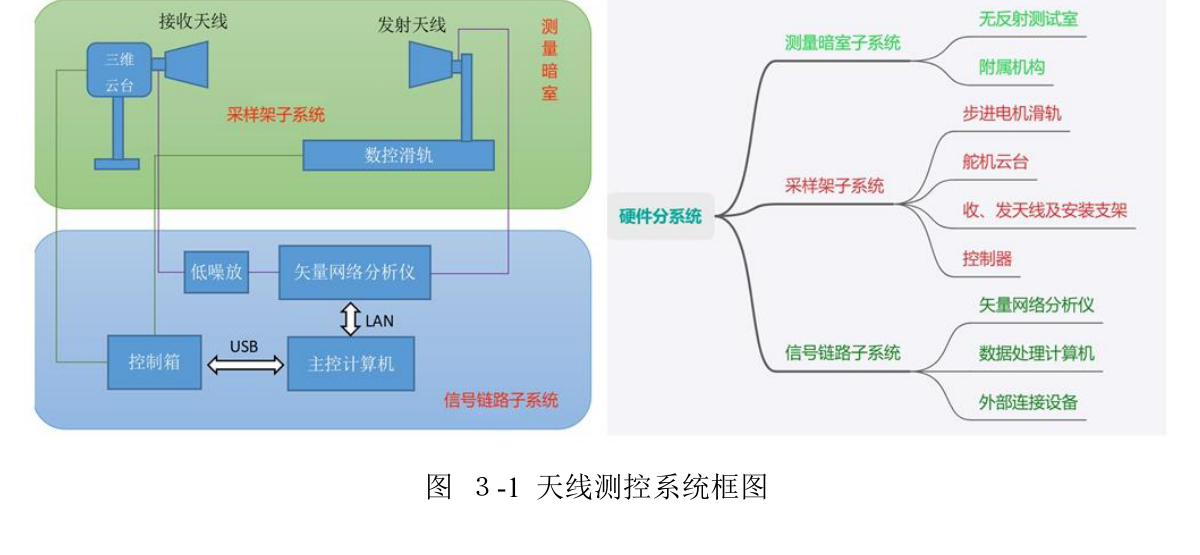
\includegraphics[width=0.78\textwidth]{figures/ref_measurement_system.png}
  \caption{天线测控系统硬件与信号链路框图}
  \label{fig:measurement-system}
\end{figure}

实验用发射、接收喇叭天线的口径尺寸如图 \ref{fig:horn-dimensions} 所示。后续理论计算中，发射天线取 $D_E=3.7\,\mathrm{cm}$、$D_H=8.2\,\mathrm{cm}$，接收天线取 $D_E=10.5\,\mathrm{cm}$、$D_H=14.1\,\mathrm{cm}$。

\begin{figure}[H]
  \centering
  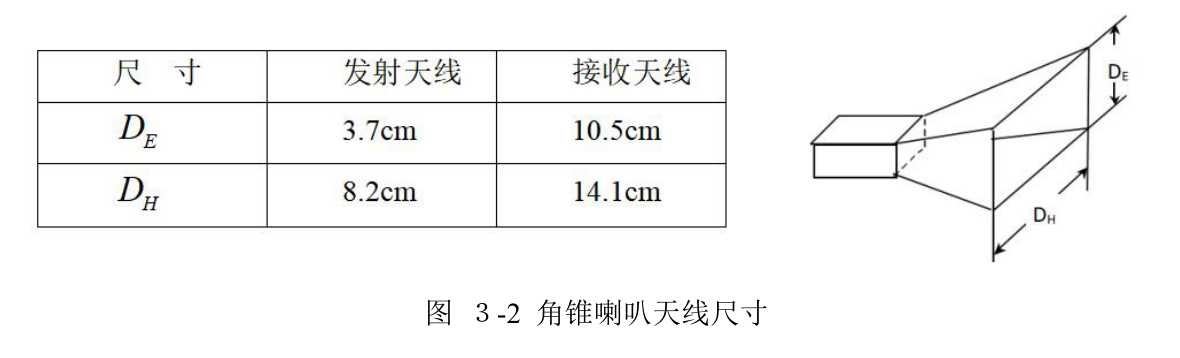
\includegraphics[width=0.72\textwidth]{figures/ref_horn_dimensions.png}
  \caption{实验用角锥喇叭天线尺寸}
  \label{fig:horn-dimensions}
\end{figure}

\subsection{$S$ 参数、驻波比与回波损耗}

天线端口与馈线不完全匹配时，入射波的一部分被天线吸收并辐射，另一部分沿馈线反射回来。端口反射系数定义为反射波与入射波幅度之比，记为 $\Gamma$。电压驻波比与反射系数之间满足
\begin{equation}
  \mathrm{VSWR}=\frac{1+|\Gamma|}{1-|\Gamma|},
  \label{eq:vswr}
\end{equation}
因此
\begin{equation}
  |\Gamma|=\frac{\mathrm{VSWR}-1}{\mathrm{VSWR}+1}.
  \label{eq:gamma-vswr}
\end{equation}
回波损耗为
\begin{equation}
  RL=-20\log_{10}|\Gamma|.
  \label{eq:return-loss}
\end{equation}
VSWR 越接近 1，$|\Gamma|$ 越小，说明端口匹配越好。$S_{11}$ 反映端口反射特性；$S_{21}$ 则反映发射天线、空间传播路径与接收天线共同形成的传输特性。若矢量网络分析仪以对数幅度显示传输系数，则
\begin{equation}
  S_{21,\mathrm{dB}}=20\log_{10}|S_{21}|.
  \label{eq:s21-db}
\end{equation}

\subsection{空间传播与远场条件}

天线周围场区可分为感应近场、辐射近场和辐射远场，如图 \ref{fig:field-regions} 所示。对于矩形口径喇叭天线，实验指导书给出的工程远场条件可写为
\begin{equation}
  R_{\mathrm{ff,horn}}\gtrsim \frac{2D_HD_E}{\lambda}.
  \label{eq:far-field-horn}
\end{equation}
若按天线最大线度 $D$ 采用更保守的远场判据，则有
\begin{equation}
  R_{\mathrm{ff}}\gtrsim \frac{2D^2}{\lambda}.
  \label{eq:far-field}
\end{equation}
当测量距离进入远场后，方向图形状趋于稳定，弗里斯传输公式可用于估算收发功率关系：
\begin{equation}
  \frac{P_r}{P_t}=\left(\frac{\lambda}{4\pi R}\right)^2G_tG_r,
  \label{eq:friis}
\end{equation}
其中 $P_t$ 和 $P_r$ 分别为发射、接收功率，$G_t$ 与 $G_r$ 分别为发射、接收天线增益，$R$ 为收发天线口面之间的距离。功率与 dBm 的换算为
\begin{equation}
  P(\mathrm{dBm})=10\log_{10}\frac{P(\mathrm{W})}{1\,\mathrm{mW}},\qquad
  P(\mathrm{W})=10^{P(\mathrm{dBm})/10}\times1\,\mathrm{mW}.
  \label{eq:dbm-w}
\end{equation}
增益的线性值与 dBi 的换算为
\begin{equation}
  G_{\mathrm{lin}}=10^{G_{\mathrm{dBi}}/10}.
  \label{eq:gain-linear}
\end{equation}
因此弗里斯公式也可写成 dB 形式：
\begin{equation}
  P_r(\mathrm{dBm})=P_t(\mathrm{dBm})+G_t(\mathrm{dBi})+G_r(\mathrm{dBi})
  +20\log_{10}\frac{\lambda}{4\pi R}.
  \label{eq:friis-db}
\end{equation}
理想自由空间远场中，接收功率随距离应近似服从 $1/R^2$ 衰减；实际平台上若存在近场过渡、反射、多径和背景噪声，拟合指数会偏离 2。

\begin{figure}[H]
  \centering
  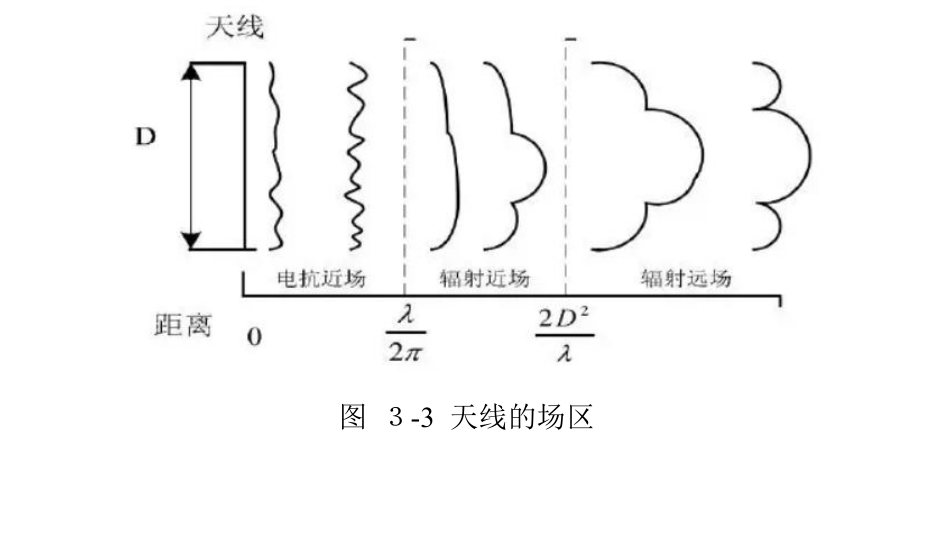
\includegraphics[width=0.58\textwidth]{figures/ref_field_regions.png}
  \caption{天线场区划分示意图}
  \label{fig:field-regions}
\end{figure}

\subsection{口径、增益与半功率波束宽度}

角锥喇叭天线的方向性主要由有效口径面积决定。若口径面积 $A_p=D_HD_E$，口径效率记为 $k$，可估算
\begin{equation}
  G\approx k\frac{4\pi A_p}{\lambda^2},\qquad
  G_{\mathrm{dBi}}=10\log_{10}G.
  \label{eq:aperture-gain}
\end{equation}
指导书给出的工程估算式相当于取 $k=0.51$；后文在和波束宽度法比较时同时列出 $k\approx1$ 的理想口径基准，用于观察实测值相对于理想上限的偏差。
发射天线的 H 面和 E 面半功率波束宽度可近似写为
\begin{equation}
  \theta_H\approx 1.18\frac{\lambda}{D_H},\qquad
  \theta_E\approx 0.89\frac{\lambda}{D_E},
  \label{eq:beamwidth-theory}
\end{equation}
其中角度初值为弧度，换算为角度后与实验方向图的 3 dB 宽度比较。

实际方向图测量中，还可用波束宽度法估算增益：
\begin{equation}
  G_{\mathrm{BW}}(\mathrm{dBi})=10\log_{10}\frac{32400}{\theta_{H,-3\mathrm{dB}}\theta_{E,-3\mathrm{dB}}},
  \label{eq:beamwidth-gain}
\end{equation}
式中 $\theta_{H,-3\mathrm{dB}}$ 和 $\theta_{E,-3\mathrm{dB}}$ 以角度为单位。

\subsection{极化测量}

线极化喇叭天线接收信号与收发天线极化方向密切相关。若发射天线极化方向相对于接收天线转过角度 $\alpha$，接收天线只能接收电场在自身极化方向上的投影。理想情况下，场幅度与 $\cos\alpha$ 成正比，功率与 $\cos^2\alpha$ 成正比。由于矢网对数幅度读数常写为 $20\log_{10}|S_{21}|$，因此常规极化曲线在 dB 坐标中应接近
\begin{equation}
  20\log_{10}|\cos\alpha|.
  \label{eq:polarization}
\end{equation}
极化栅网相当于选择性透射或反射某一方向电场分量的结构，会改变通过栅网后的有效极化方向和接收幅度。若比较同极化与交叉极化接收电平，可用轴向交叉极化隔离度表示：
\begin{equation}
  XPD=P_{\mathrm{cop}}(\mathrm{dBm})-P_{\mathrm{xp}}(\mathrm{dBm}).
  \label{eq:xpd}
\end{equation}

\section{实验设备、步骤与数据来源}

\subsection{实验设备}

实验使用天线综合测控系统、矢量网络分析仪、步进电机滑轨、舵机转台、波导角锥喇叭天线、极化栅网和可移动微波屏蔽板。测量频段为 5.0 GHz 至 8.5 GHz；方向图选取 6.5 GHz、7.5 GHz、8.5 GHz；极化和距离实验选取 8.00 GHz。

\begin{figure}[H]
  \centering
  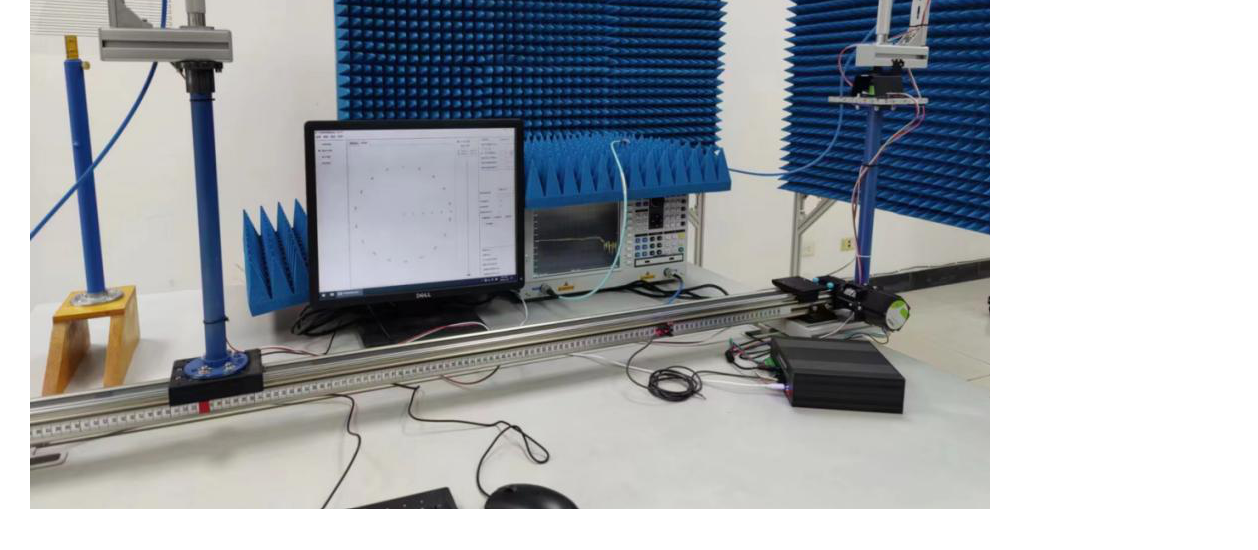
\includegraphics[width=0.82\textwidth]{figures/ref_system_photo.png}
  \caption{天线测控系统实物布置}
  \label{fig:system-photo}
\end{figure}

实物系统如图 \ref{fig:system-photo} 所示。收、发喇叭天线分别安装在滑轨两端的支架上，中间布置吸波材料以削弱墙面和桌面的反射；矢量网络分析仪提供扫频信号并读取 $S$ 参数，计算机软件控制转台角度、滑轨位移和数据保存。该布置决定了后续测量的基本约束：方向图实验应保证口面对准和极化一致，距离实验应记录滑轨位移与口面间距的关系，极化实验则要在不改变天线主轴位置的前提下旋转极化角。

\subsection{实验步骤}

本次测量按指导书给出的项目顺序进行，具体步骤如下。

\begin{enumerate}
  \item \textbf{实验前准备与回零。} 在控制器通电前，先确认接收天线位于滑轨光电检测传感器左侧，避免开机后滑轨和舵机被锁定而无法手动调整。随后打开控制器电源，使接收天线向发射端移动并完成零点定位；检查矢量网络分析仪、控制器、计算机和两副喇叭天线之间的连接。
  \item \textbf{软件连接与姿态校准。} 打开天线测控软件，依次连接天线控制器和矢量网络分析仪，确认通信端口和仪器状态正常。利用调试界面微调收发喇叭的方位角、高度和极化方向，使两副天线口面相对、主轴基本共线，并使同极化方向对应。
  \item \textbf{$S_{11}$ 驻波比测量。} 在 $S$ 参数测量界面选择 $S_{11}$，频率范围设为 5.0--8.5 GHz，显示量选择 VSWR。完成扫频后保存 CSV 文件，同时保留测控软件界面图片，用于后续核对曲线形状和坐标设置。
  \item \textbf{$S_{21}$ 传输测量。} 保持收发天线对准和同极化，在同一频段内测量 $S_{21}$ 对数幅度。该曲线用于判断空间链路在不同频率下的传输稳定性，并为方向图、极化和距离测量选择合适频点提供依据。
  \item \textbf{水平面和垂直面方向图测量。} 进入辐射方向图测量界面，分别选择水平面和垂直面极坐标扫描。扫描频点设为 6.5 GHz、7.5 GHz 和 8.5 GHz，角度范围取 $-135^\circ$ 至 $135^\circ$，步进角为 $2^\circ$。每次扫描前重新确认主瓣方向附近没有人员遮挡，并保持吸波材料位置不变。
  \item \textbf{极化特性测量。} 固定工作频率 8.00 GHz 和收发天线间距，改变接收端相对极化角，记录 $0^\circ$ 至 $90^\circ$ 范围内的传输幅度。完成常规极化曲线后，在天线间加入极化栅网并重复测量，用于比较栅网对透射幅度和等效极化方向的影响。
  \item \textbf{距离传播特性测量。} 固定频率 8.00 GHz、天线极化和方位角，沿滑轨改变接收天线位置。实验中记录滑轨位移并导出接收信号曲线，后续以口面间距 $R=R_0+x$ 对接收功率进行幂律拟合。
  \item \textbf{数据导出与复核。} 每个项目结束后导出 CSV 数据，并保存软件界面图片。数据处理时先检查 CSV 与界面记录中的频率、角度和距离范围是否一致，再进行归一化、单位换算、半功率点插值和幂律拟合。
\end{enumerate}

实验原始界面记录如图 \ref{fig:raw-screenshots-sparam} 至图 \ref{fig:raw-screenshots-distance} 所示。这些图片用于记录软件设置和原始曲线状态；后续分析曲线按导出的 CSV 数据重新绘制。

\begin{figure}[H]
  \centering
  \begin{subfigure}[b]{0.48\textwidth}
    \centering
    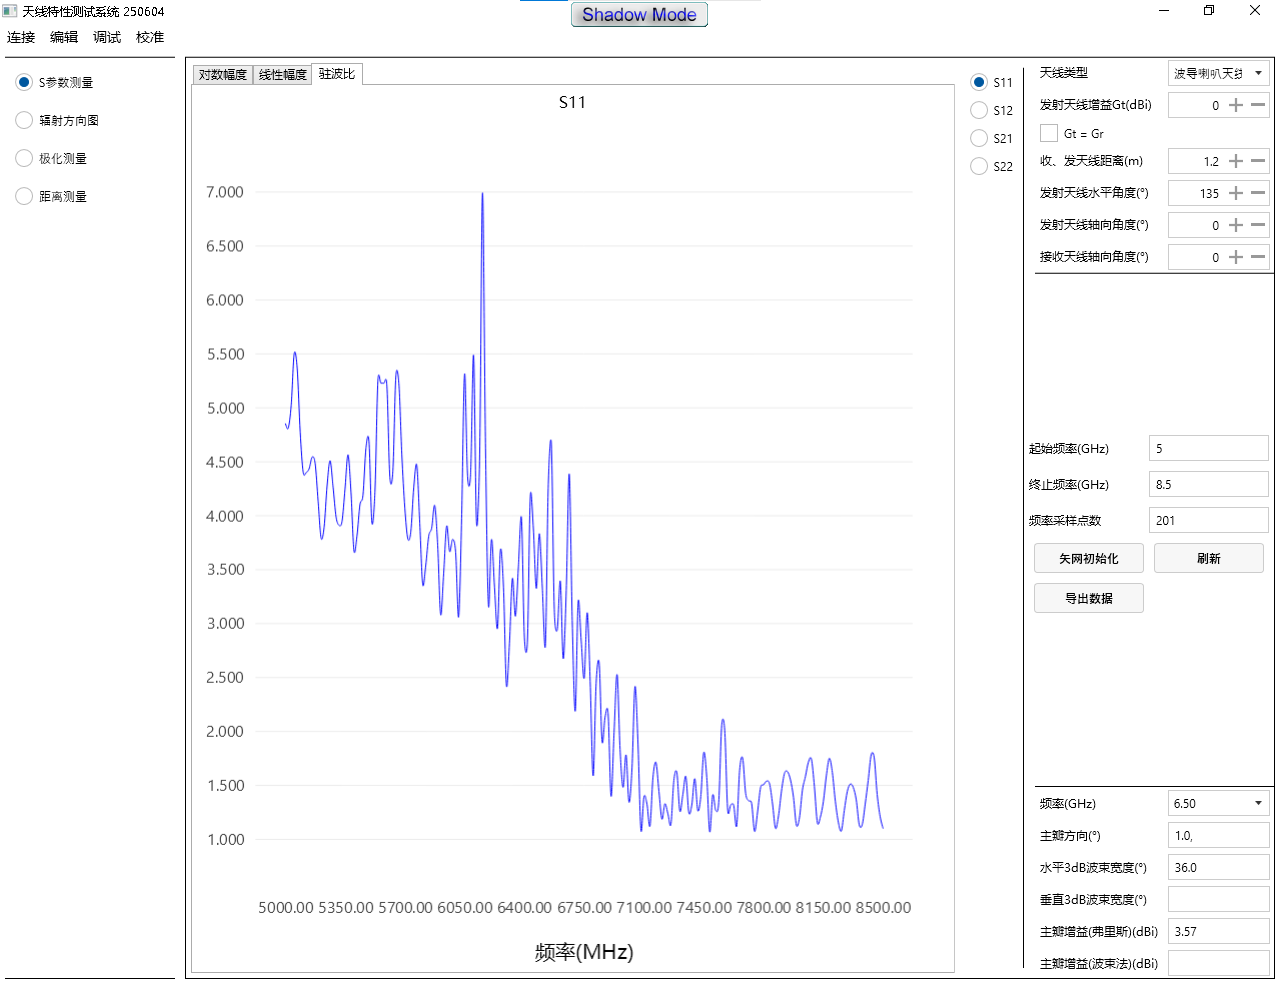
\includegraphics[width=\textwidth]{figures/raw_s11_screenshot.png}
    \caption{$S_{11}$ 驻波比测量界面}
  \end{subfigure}
  \hfill
  \begin{subfigure}[b]{0.48\textwidth}
    \centering
    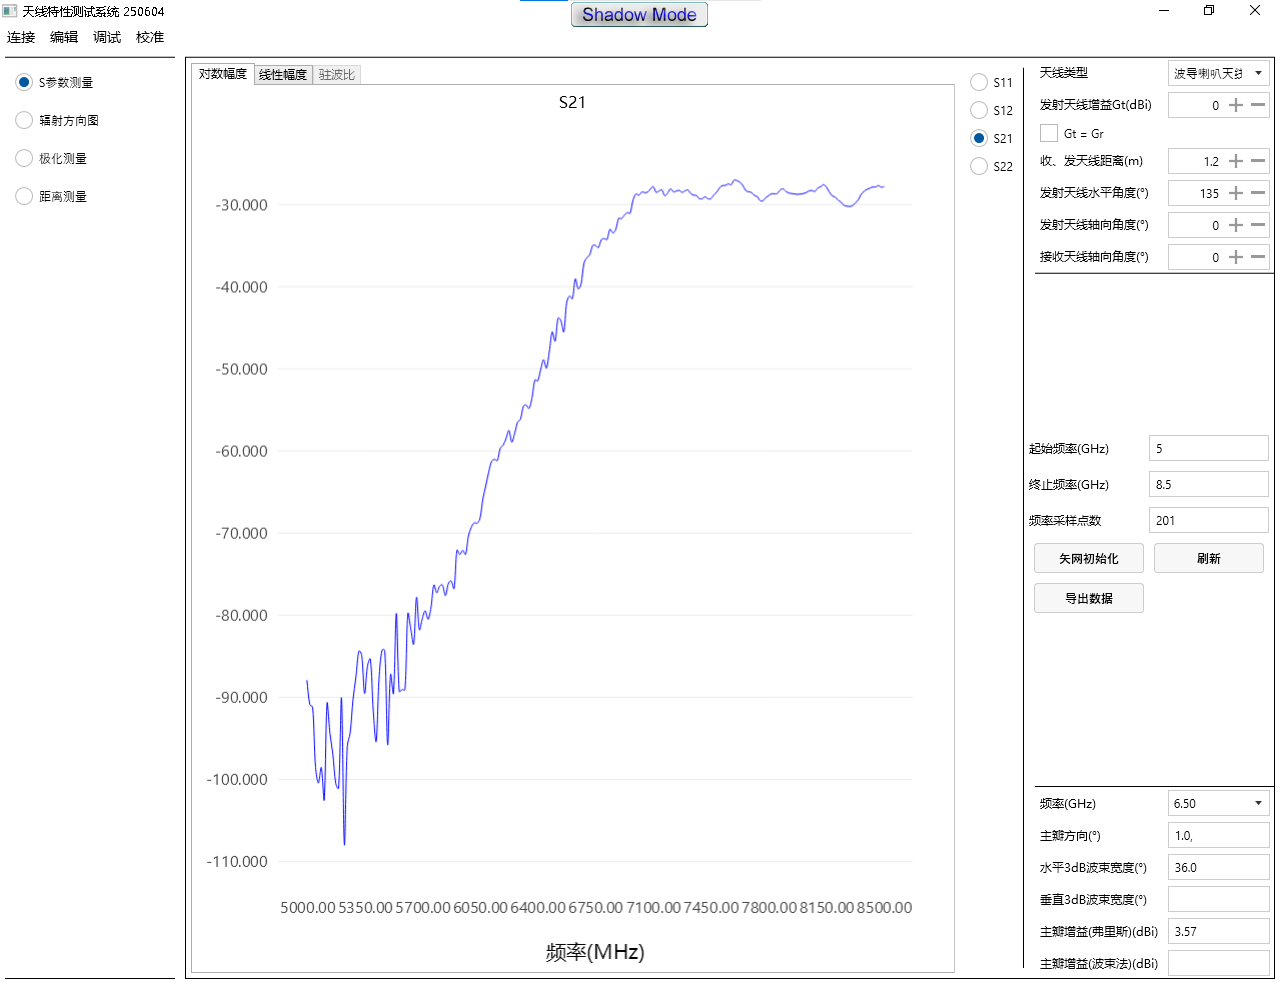
\includegraphics[width=\textwidth]{figures/raw_s21_screenshot.png}
    \caption{$S_{21}$ 传输测量界面}
  \end{subfigure}
  \caption{$S$ 参数测量原始界面}
  \label{fig:raw-screenshots-sparam}
\end{figure}

\begin{figure}[H]
  \centering
  \begin{subfigure}[b]{0.48\textwidth}
    \centering
    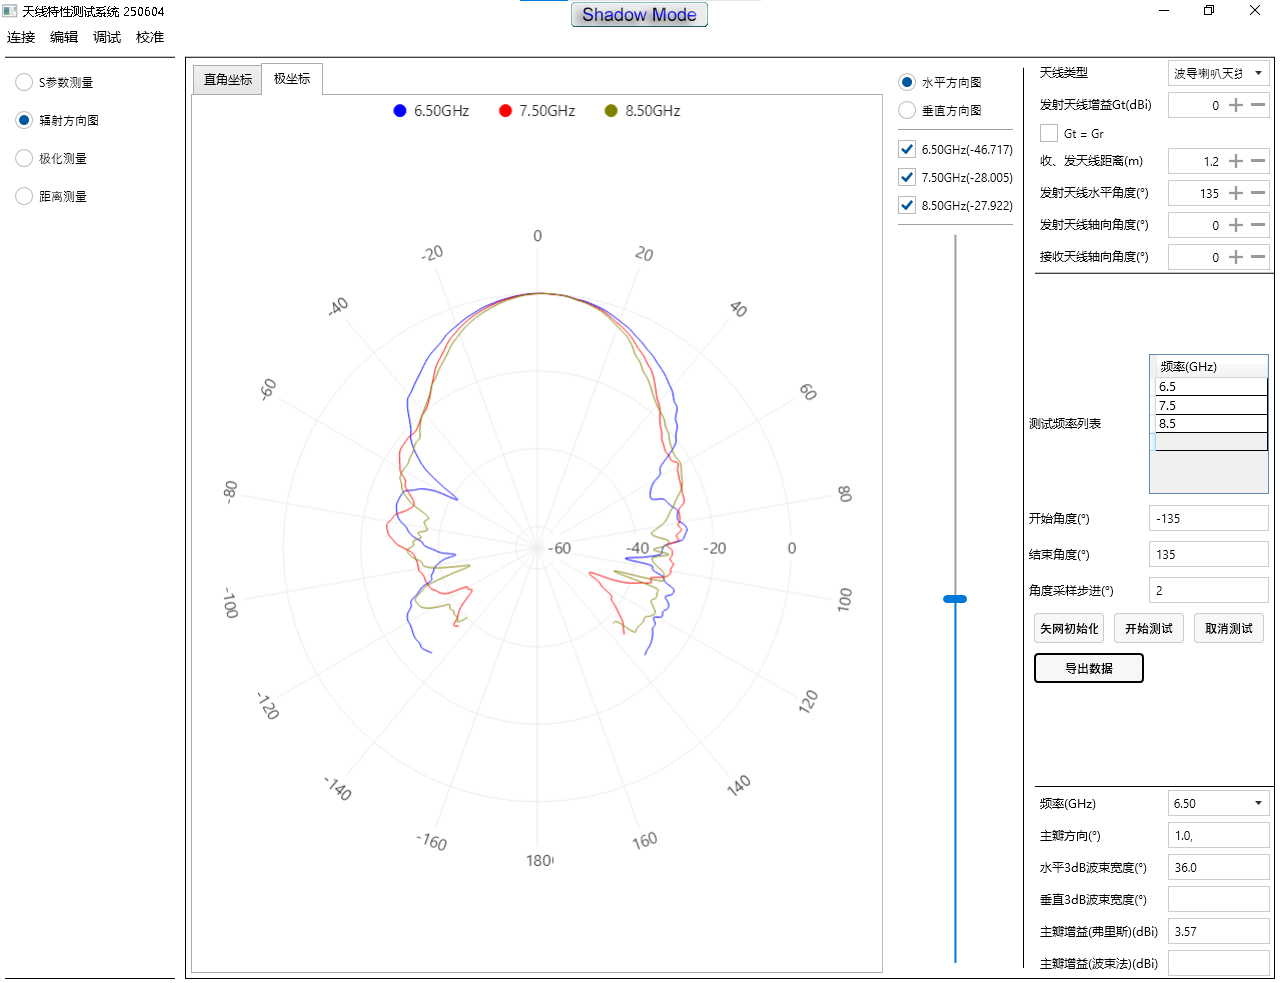
\includegraphics[width=\textwidth]{figures/raw_hplane_screenshot.png}
    \caption{水平面方向图测量界面}
  \end{subfigure}
  \hfill
  \begin{subfigure}[b]{0.48\textwidth}
    \centering
    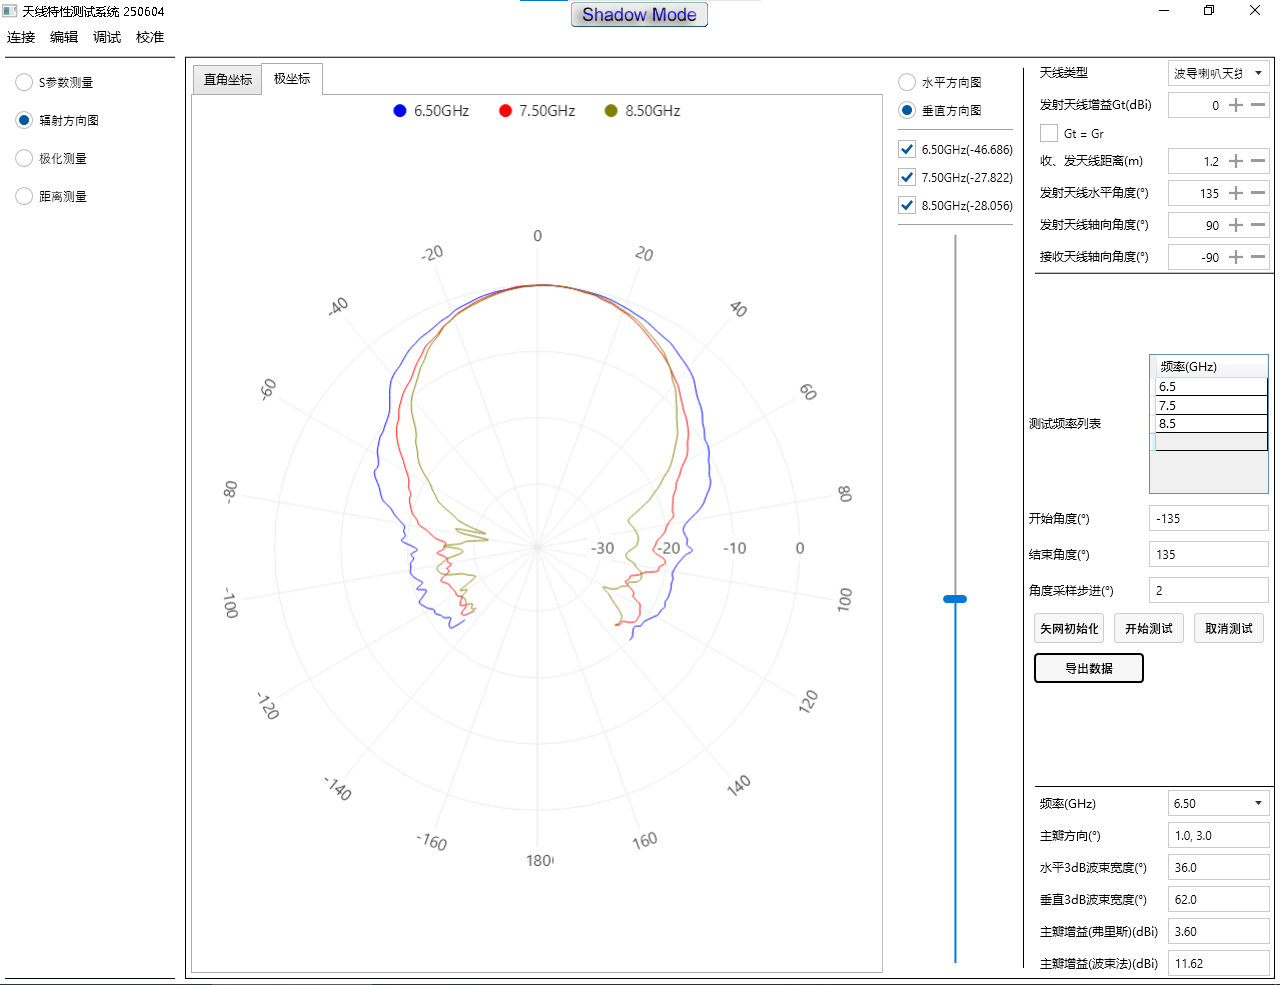
\includegraphics[width=\textwidth]{figures/raw_eplane_screenshot.png}
    \caption{垂直面方向图测量界面}
  \end{subfigure}
  \caption{方向图测量原始界面}
  \label{fig:raw-screenshots-pattern}
\end{figure}

\begin{figure}[H]
  \centering
  \begin{subfigure}[b]{0.32\textwidth}
    \centering
    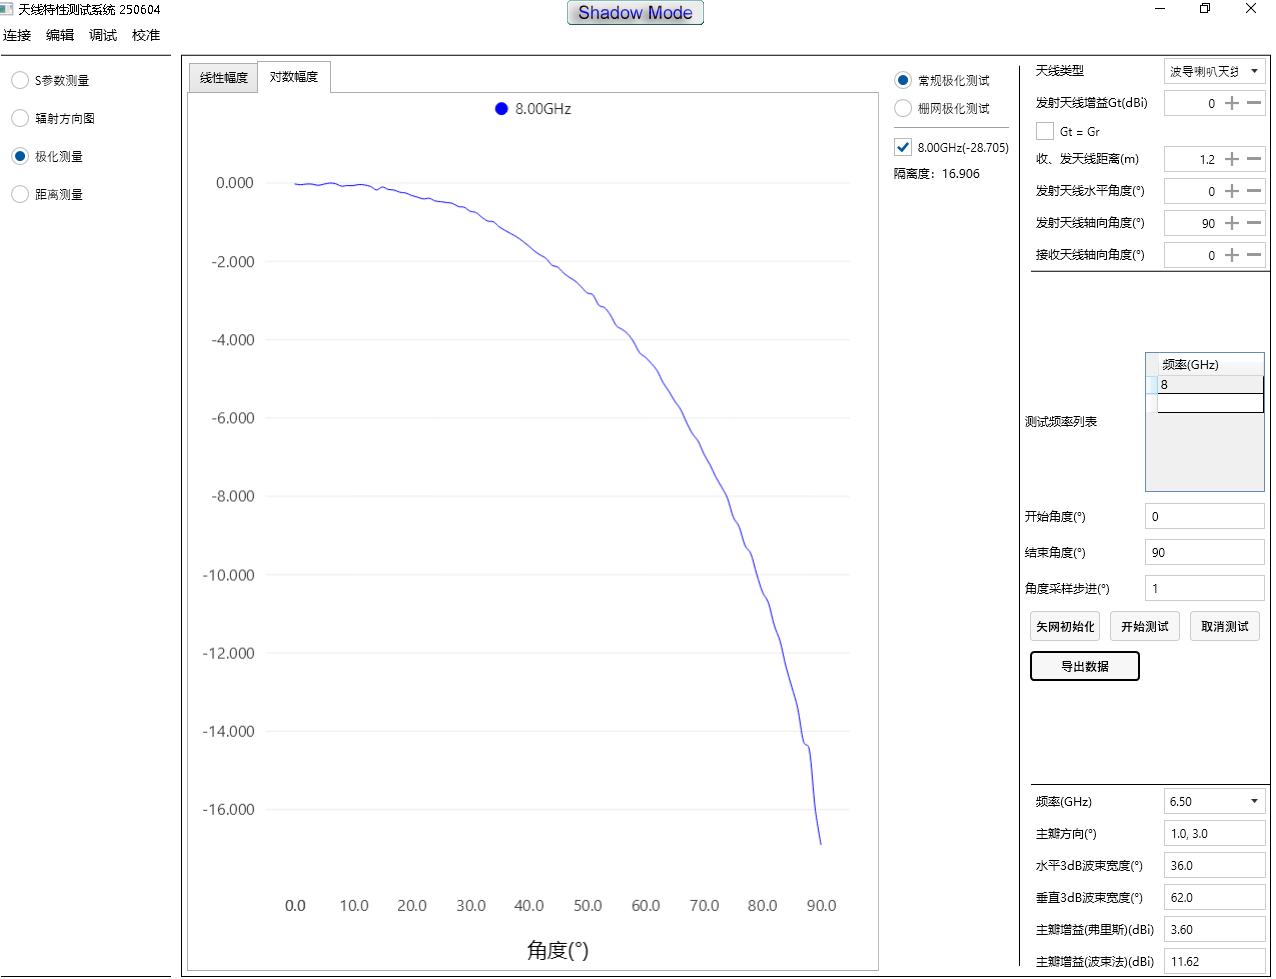
\includegraphics[width=\textwidth]{figures/raw_polarization_screenshot.png}
    \caption{常规极化}
  \end{subfigure}
  \hfill
  \begin{subfigure}[b]{0.32\textwidth}
    \centering
    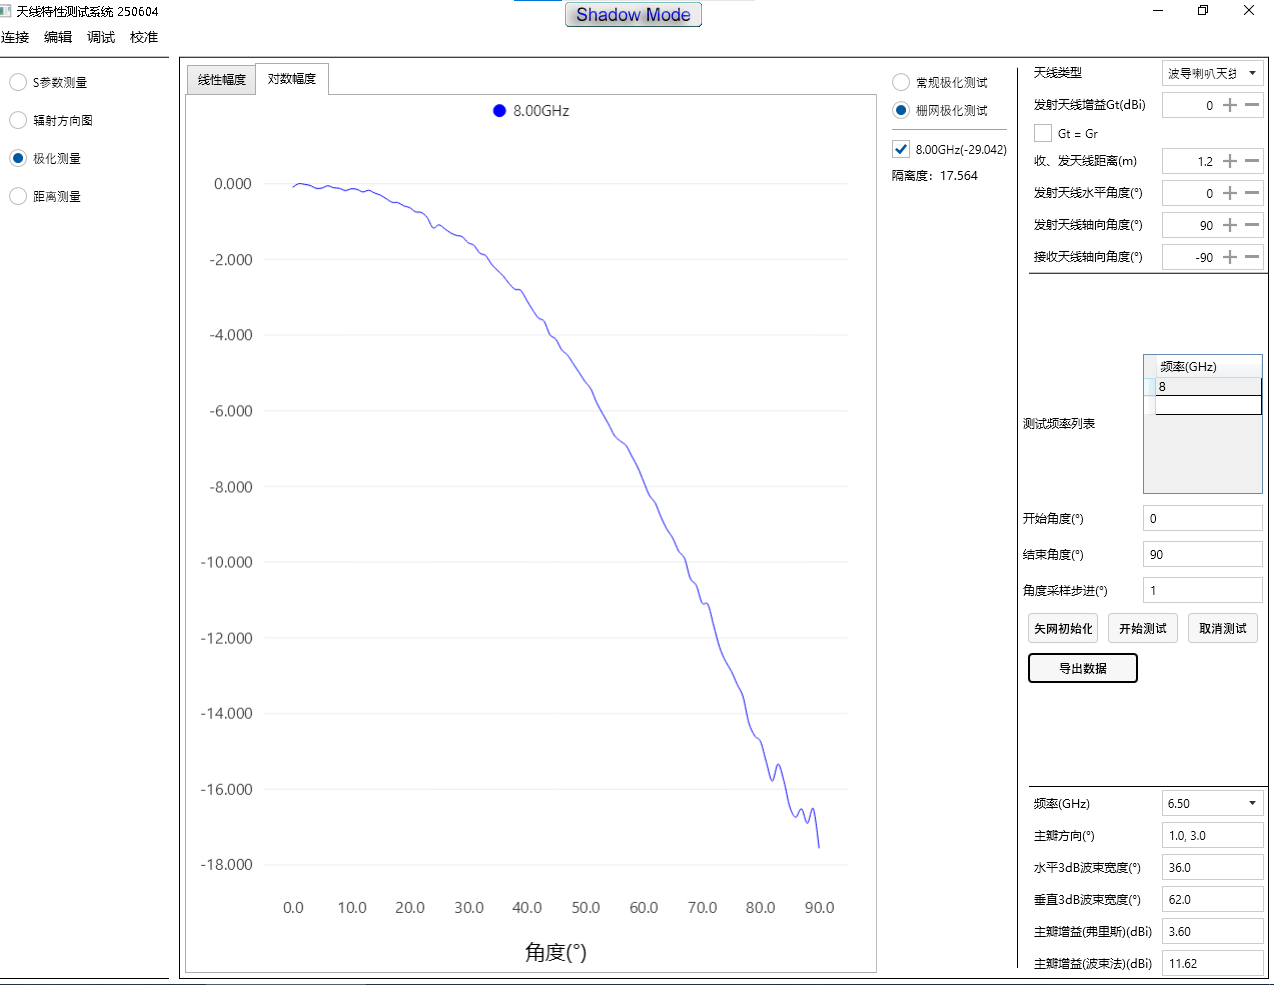
\includegraphics[width=\textwidth]{figures/raw_grid_polarization_screenshot.png}
    \caption{加栅网极化}
  \end{subfigure}
  \hfill
  \begin{subfigure}[b]{0.32\textwidth}
    \centering
    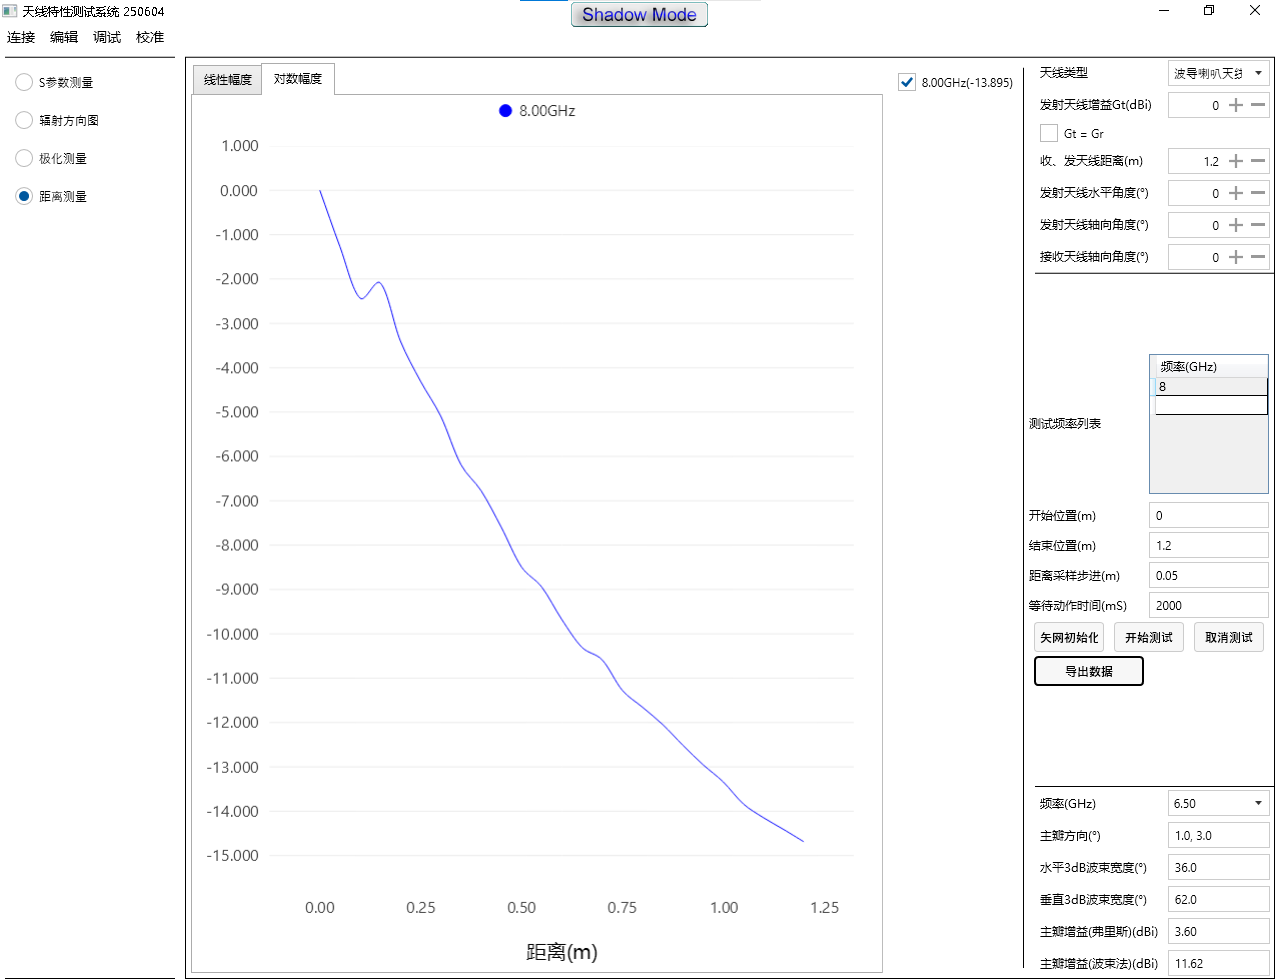
\includegraphics[width=\textwidth]{figures/raw_distance_screenshot.png}
    \caption{距离测量}
  \end{subfigure}
  \caption{极化和距离测量原始界面}
  \label{fig:raw-screenshots-distance}
\end{figure}

\subsection{数据处理方法}

本文曲线图以实验导出的 CSV 文件为基础重新绘制。$S_{11}$ 数据中的 VSWR 按式 \eqref{eq:gamma-vswr} 和式 \eqref{eq:return-loss} 换算 $|\Gamma|$ 与回波损耗；方向图数据先以各频点最大值归一化，再提取主瓣附近的 $-3\,\mathrm{dB}$ 交点；极化数据用归一化 $S_{21}$ 幅度和对数幅度同时判断；距离数据以 $R=R_0+x$ 建模，其中 $x$ 为滑轨位移，参照实验平台几何取 $R_0=0.55\,\mathrm{m}$。表格仅列典型频点或提取参数，完整采样点均参与相应曲线绘制和拟合。

\section{实验数据与分析}

\subsection{$S_{11}$ 与 $S_{21}$ 扫频结果}

图 \ref{fig:s-parameter-sweep} 给出了重新绘制的 $S_{11}$ 驻波比和 $S_{21}$ 对数幅度曲线。由表 \ref{tab:s-parameters} 可见，低频端 6.5 GHz 的 VSWR 为 3.332，回波损耗仅 5.38 dB，端口匹配较差；频率升高后匹配明显改善，7.485 GHz 处 VSWR 达到最小值 1.069，对应 $|\Gamma|=0.0333$、回波损耗 29.54 dB。8.5 GHz 处 VSWR 为 1.099，仍保持良好匹配。

$S_{21}$ 曲线在 7 GHz 以下迅速上升，7.0 GHz 以后进入较平坦的传输区。实测最大值出现在 7.590 GHz，约为 $-27.021\,\mathrm{dB}$；7.5 GHz 至 8.5 GHz 区间的 $S_{21}$ 大多维持在 $-28\,\mathrm{dB}$ 附近。这说明在本实验收发距离和天线姿态下，高频端空间链路更稳定，适合作为方向图、极化和距离测量的工作频段。

\begin{figure}[H]
  \centering
  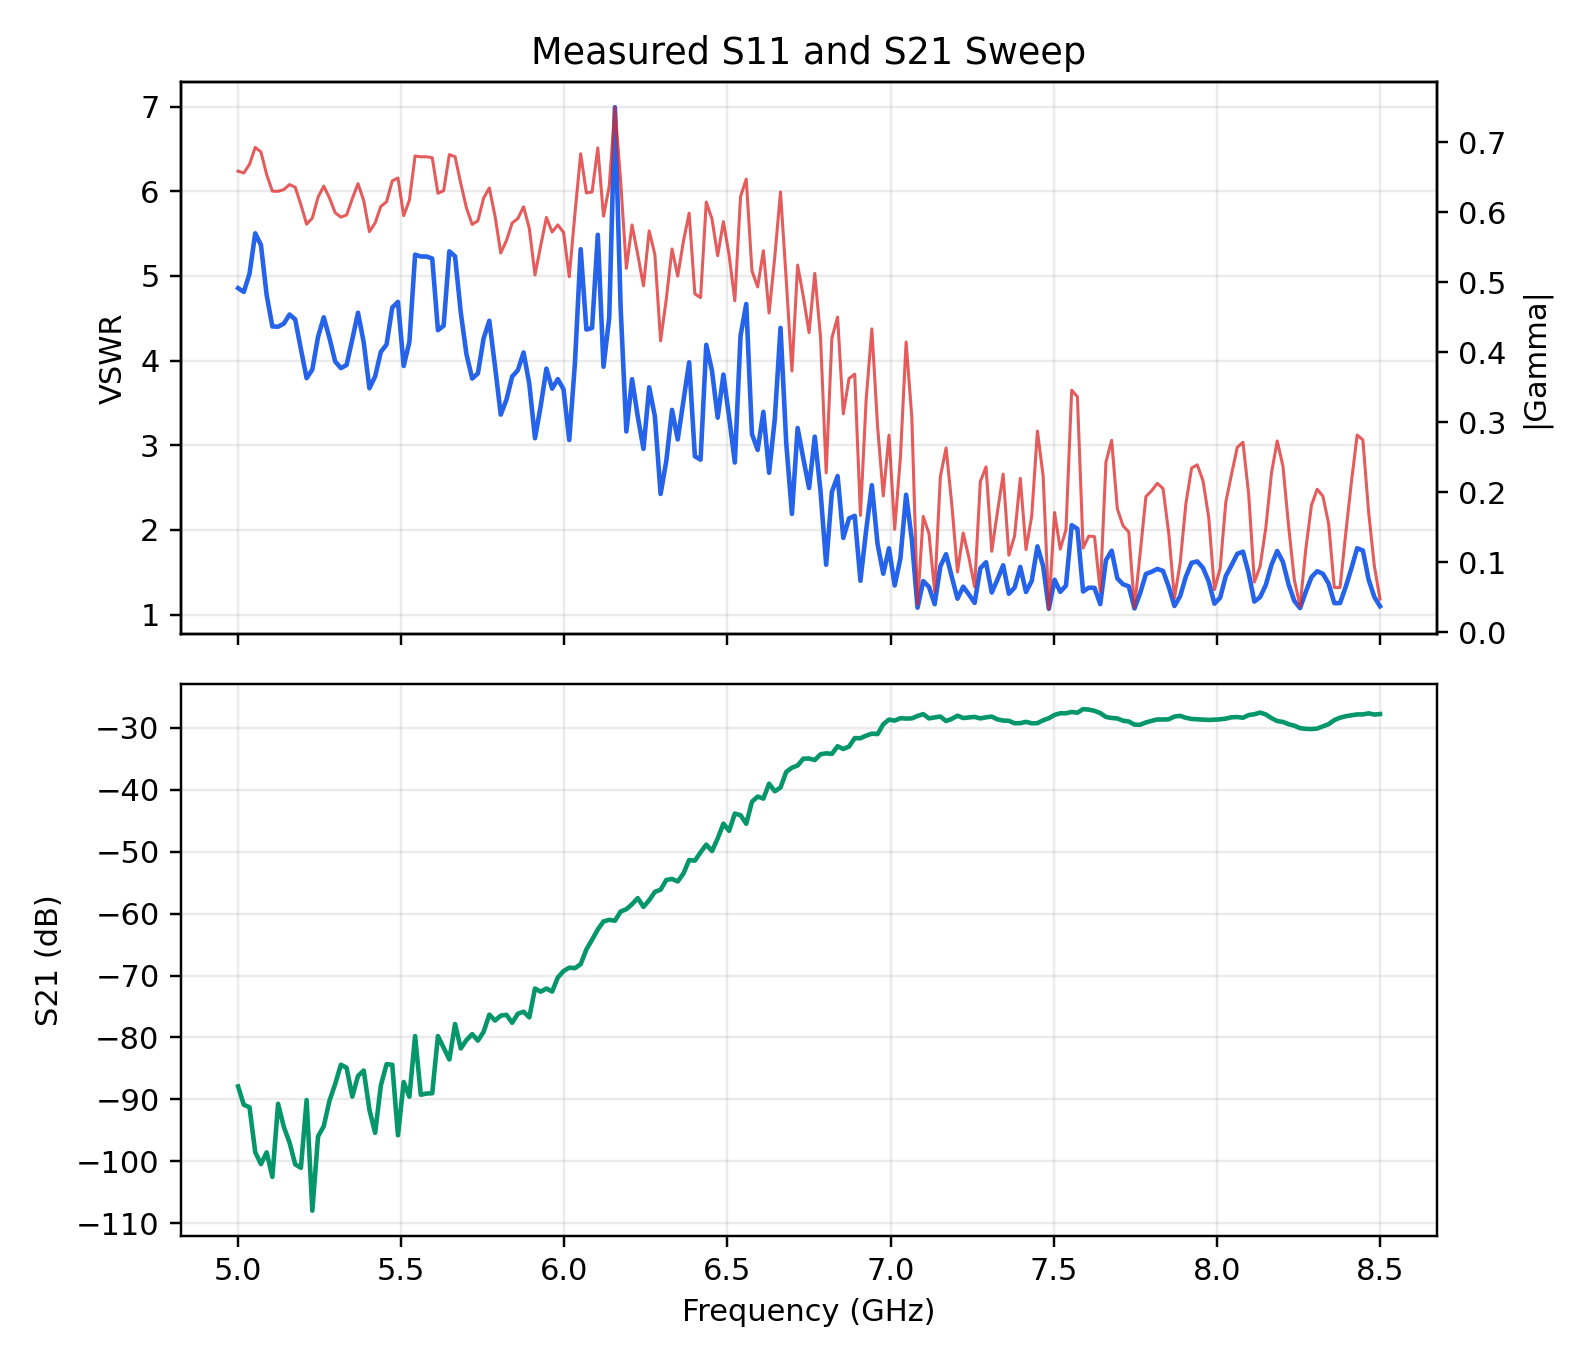
\includegraphics[width=0.78\textwidth]{figures/s_parameter_sweep.png}
  \caption{发射喇叭天线 $S_{11}$ 驻波比和收发链路 $S_{21}$ 扫频结果}
  \label{fig:s-parameter-sweep}
\end{figure}

\begin{table}[H]
  \centering
  \caption{$S_{11}$ 与 $S_{21}$ 典型频点数据}
  \label{tab:s-parameters}
  \small
  \begin{tabular}{ccccc}
    \toprule
    频率/GHz & VSWR & $|\Gamma|$ & 回波损耗/dB & $S_{21}$/dB \\
    \midrule
    6.5 & 3.332 & 0.538 & 5.38 & -46.653 \\
    7.5 & 1.412 & 0.171 & 15.35 & -27.956 \\
    8.0 & 1.129 & 0.061 & 24.35 & -28.720 \\
    8.5 & 1.099 & 0.047 & 26.53 & -27.816 \\
    \bottomrule
  \end{tabular}
\end{table}

\subsection{水平面与垂直面辐射方向图}

图 \ref{fig:pattern-results} 为水平面与垂直面方向图。三组曲线的主瓣均位于 $0^\circ$ 附近，说明收发天线主轴对准较好。随着频率从 6.5 GHz 升高到 8.5 GHz，水平面半功率波束宽度由 $34.47^\circ$ 减小到 $28.45^\circ$，体现了口径尺寸相对波长增大后方向性增强的趋势。垂直面波束宽度整体大于水平面，这与发射喇叭天线的 $D_E$ 小于 $D_H$ 相符。

\begin{figure}[H]
  \centering
  \begin{subfigure}[b]{0.48\textwidth}
    \centering
    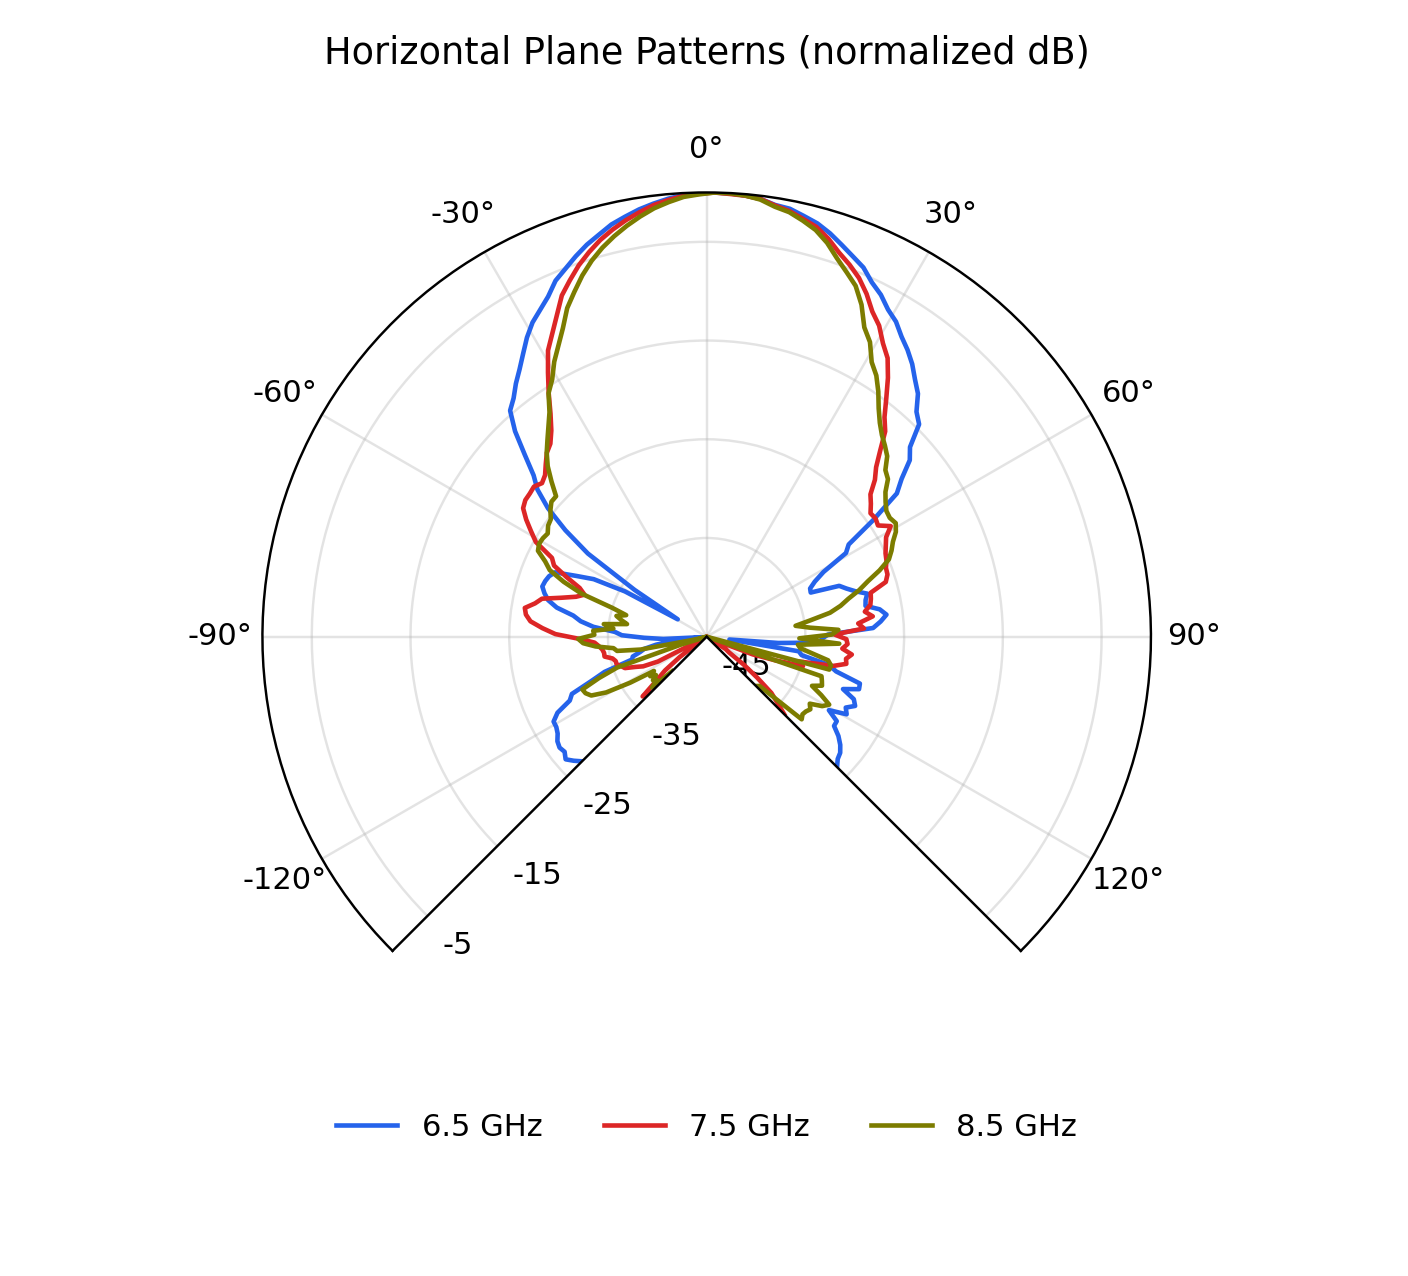
\includegraphics[width=\textwidth]{figures/h_plane_patterns.png}
    \caption{水平面方向图}
  \end{subfigure}
  \hfill
  \begin{subfigure}[b]{0.48\textwidth}
    \centering
    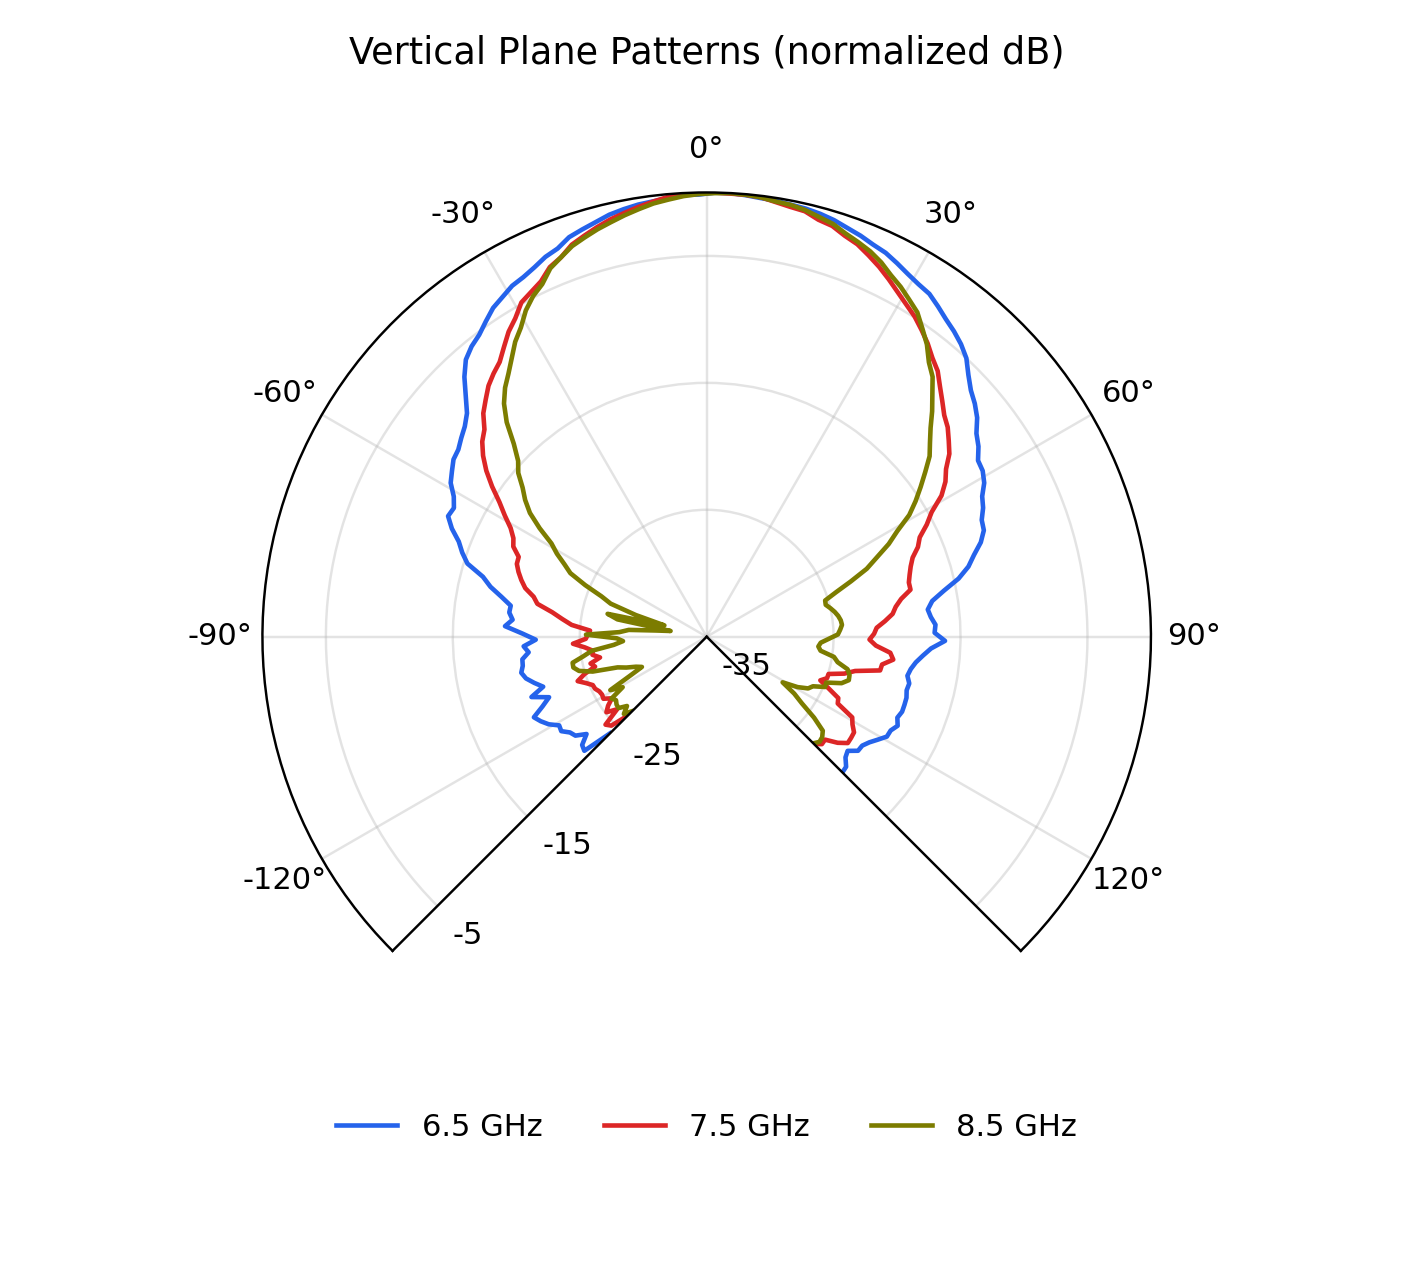
\includegraphics[width=\textwidth]{figures/e_plane_patterns.png}
    \caption{垂直面方向图}
  \end{subfigure}
  \caption{发射喇叭天线水平面与垂直面极坐标方向图（各频点按最大值归一化）}
  \label{fig:pattern-results}
\end{figure}

\begin{table}[H]
  \centering
  \caption{方向图实测主瓣方向、半功率波束宽度与波束宽度法增益}
  \label{tab:pattern-results}
  \small
  \begin{tabular}{cccccc}
    \toprule
    频率/GHz & H 面主瓣/$^\circ$ & H 面 HPBW/$^\circ$ & E 面主瓣/$^\circ$ & E 面 HPBW/$^\circ$ & $G_{\mathrm{BW}}$/dBi \\
    \midrule
    6.5 & 1.0 & 34.47 & 3.0 & 59.66 & 11.97 \\
    7.5 & 1.0 & 31.24 & 1.0 & 46.65 & 13.47 \\
    8.5 & 1.0 & 28.45 & 3.0 & 47.98 & 13.75 \\
    \bottomrule
  \end{tabular}
\end{table}

利用式 \eqref{eq:beamwidth-theory} 可计算发射喇叭天线理论半功率宽度，结果如表 \ref{tab:beamwidth-compare} 所示。H 面理论与实测吻合较好，尤其在 8.5 GHz 处理论值 $29.10^\circ$ 与实测值 $28.45^\circ$ 接近。E 面在 6.5 GHz 与 8.5 GHz 附近也接近理论估计，7.5 GHz 处实测值偏小，可能与采样步进、局部反射、屏蔽板位置和主瓣两侧曲线不完全对称有关。总体来看，主瓣宽度随频率升高而减小的趋势与理论一致。

\begin{table}[H]
  \centering
  \caption{发射喇叭天线理论与实测半功率波束宽度对比}
  \label{tab:beamwidth-compare}
  \small
  \begin{tabular}{ccccc}
    \toprule
    频率/GHz & H 面理论/$^\circ$ & H 面实测/$^\circ$ & E 面理论/$^\circ$ & E 面实测/$^\circ$ \\
    \midrule
    6.5 & 38.05 & 34.47 & 63.61 & 59.66 \\
    7.5 & 32.98 & 31.24 & 55.13 & 46.65 \\
    8.5 & 29.10 & 28.45 & 48.64 & 47.98 \\
    \bottomrule
  \end{tabular}
\end{table}

\subsection{极化特性测量}

图 \ref{fig:polarization} 给出了 8.00 GHz 常规极化曲线和加极化栅网后的曲线。常规测量中，$\alpha=0^\circ$ 附近信号最大，$\alpha=90^\circ$ 时信号降至约 $-17.08\,\mathrm{dB}$，体现出线极化天线的交叉极化抑制能力。曲线整体接近 $20\log_{10}|\cos\alpha|$ 的形状，但在大角度处衰减没有理想曲线那么深，这与天线交叉极化分量、暗室反射和接收机噪声底有关。

加极化栅网后，曲线在 $45^\circ$ 至 $80^\circ$ 区间下降更快。例如 $\alpha=45^\circ$ 时，常规测量为 $-2.16\,\mathrm{dB}$，加栅网后为 $-4.15\,\mathrm{dB}$；$\alpha=80^\circ$ 时分别为 $-10.46\,\mathrm{dB}$ 和 $-14.89\,\mathrm{dB}$。这说明栅网不仅改变投影关系，还引入了额外透射损耗和散射。

\begin{figure}[H]
  \centering
  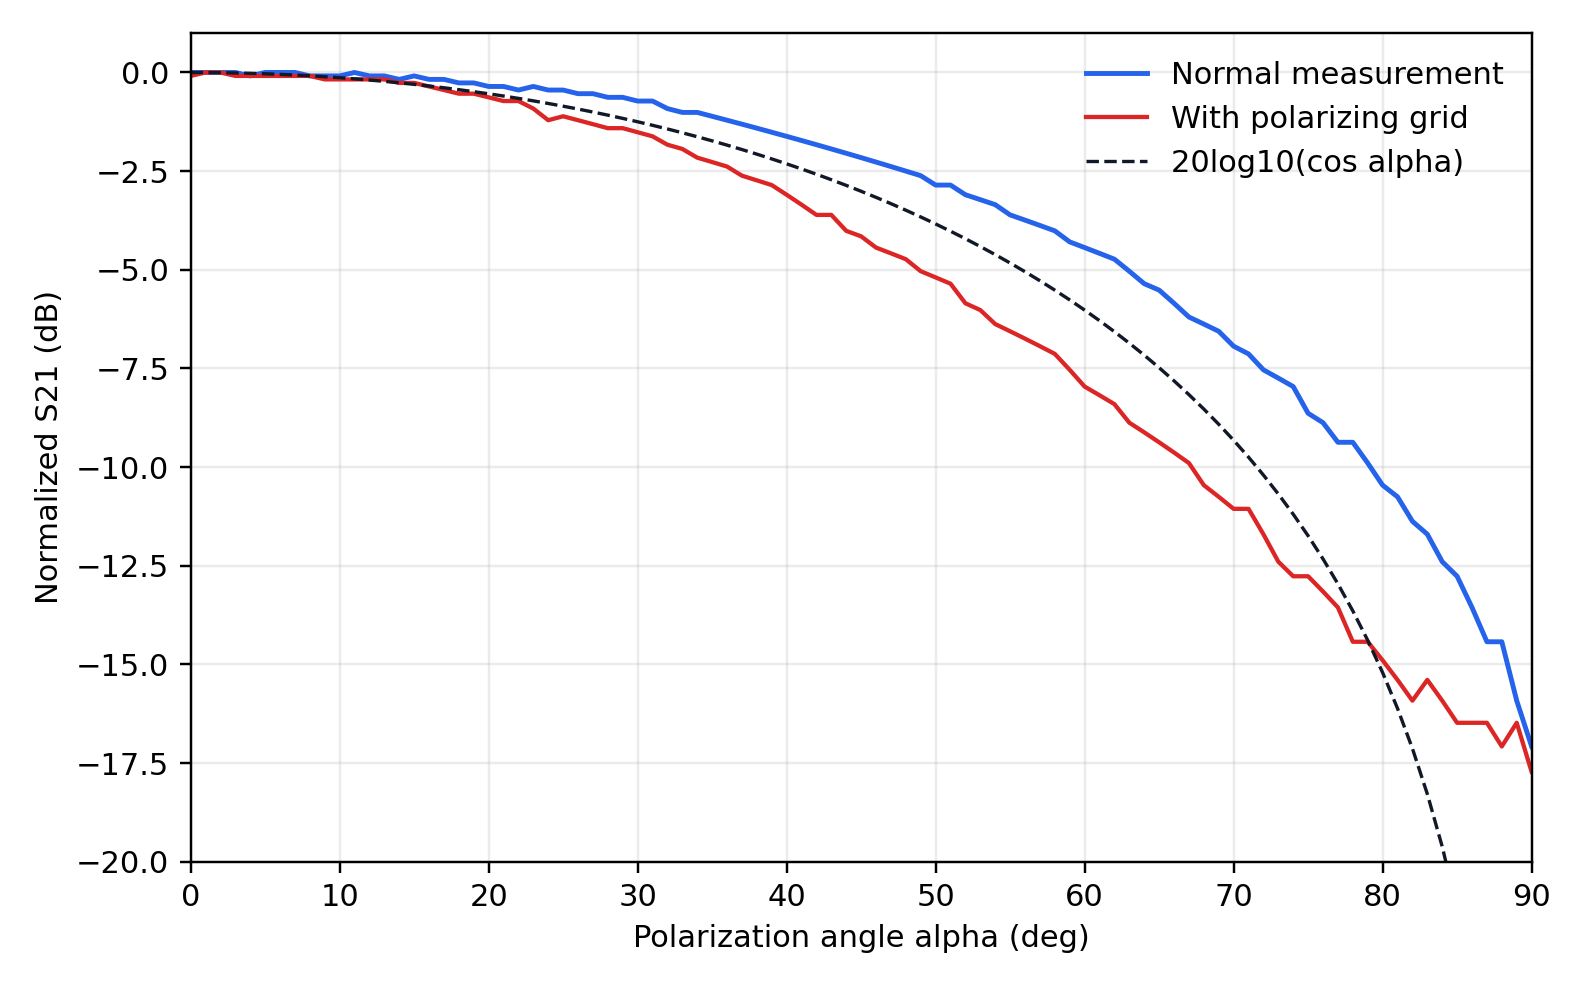
\includegraphics[width=0.74\textwidth]{figures/polarization_curves.png}
  \caption{8.00 GHz 极化曲线与理想 $20\log_{10}|\cos\alpha|$ 曲线对比}
  \label{fig:polarization}
\end{figure}

\begin{table}[H]
  \centering
  \caption{极化测量典型角度读数}
  \label{tab:polarization}
  \small
  \begin{tabular}{ccccc}
    \toprule
    极化角/$^\circ$ & 常规幅度 & 常规/dB & 栅网幅度 & 栅网/dB \\
    \midrule
    0 & 1.00 & 0.00 & 0.99 & -0.09 \\
    30 & 0.92 & -0.72 & 0.84 & -1.51 \\
    45 & 0.78 & -2.16 & 0.62 & -4.15 \\
    60 & 0.60 & -4.44 & 0.40 & -7.96 \\
    80 & 0.30 & -10.46 & 0.18 & -14.89 \\
    90 & 0.14 & -17.08 & 0.13 & -17.72 \\
    \bottomrule
  \end{tabular}
\end{table}

按式 \eqref{eq:xpd} 估算，常规测量中 $0^\circ$ 与 $90^\circ$ 的接收电平相差约 $17.08\,\mathrm{dB}$；加入极化栅网后对应差值约 $17.63\,\mathrm{dB}$。这两个数值都说明实际系统存在有限的交叉极化泄漏和噪声底，因此大角度处不会像理想 $\cos\alpha$ 曲线那样继续下降到负无穷。

从物理量角度看，矢网记录的归一化 $|S_{21}|$ 更接近场幅度投影，因此随角度近似服从 $\cos\alpha$；若讨论接收功率，则应写为 $P_r\propto |S_{21}|^2\propto \cos^2\alpha$。因此“功率随极化角变化”的理论关系应为 $\cos^2\alpha$，而 dB 坐标中表现为式 \eqref{eq:polarization}。

\subsection{距离传播特性}

图 \ref{fig:distance-fit} 将 8.00 GHz 距离测量结果与 $1/R$、$1/R^2$ 和 $1/R^3$ 曲线进行了比较。实验中以 $R=0.55+x$ 估算收发口面间距离，最小二乘拟合得到功率衰减指数 $n\approx2.96$，明显更接近 $1/R^3$。若按理想自由空间远场传播，应更接近 $1/R^2$；本实验偏快衰减说明测量条件并非理想无限自由空间。

\begin{figure}[H]
  \centering
  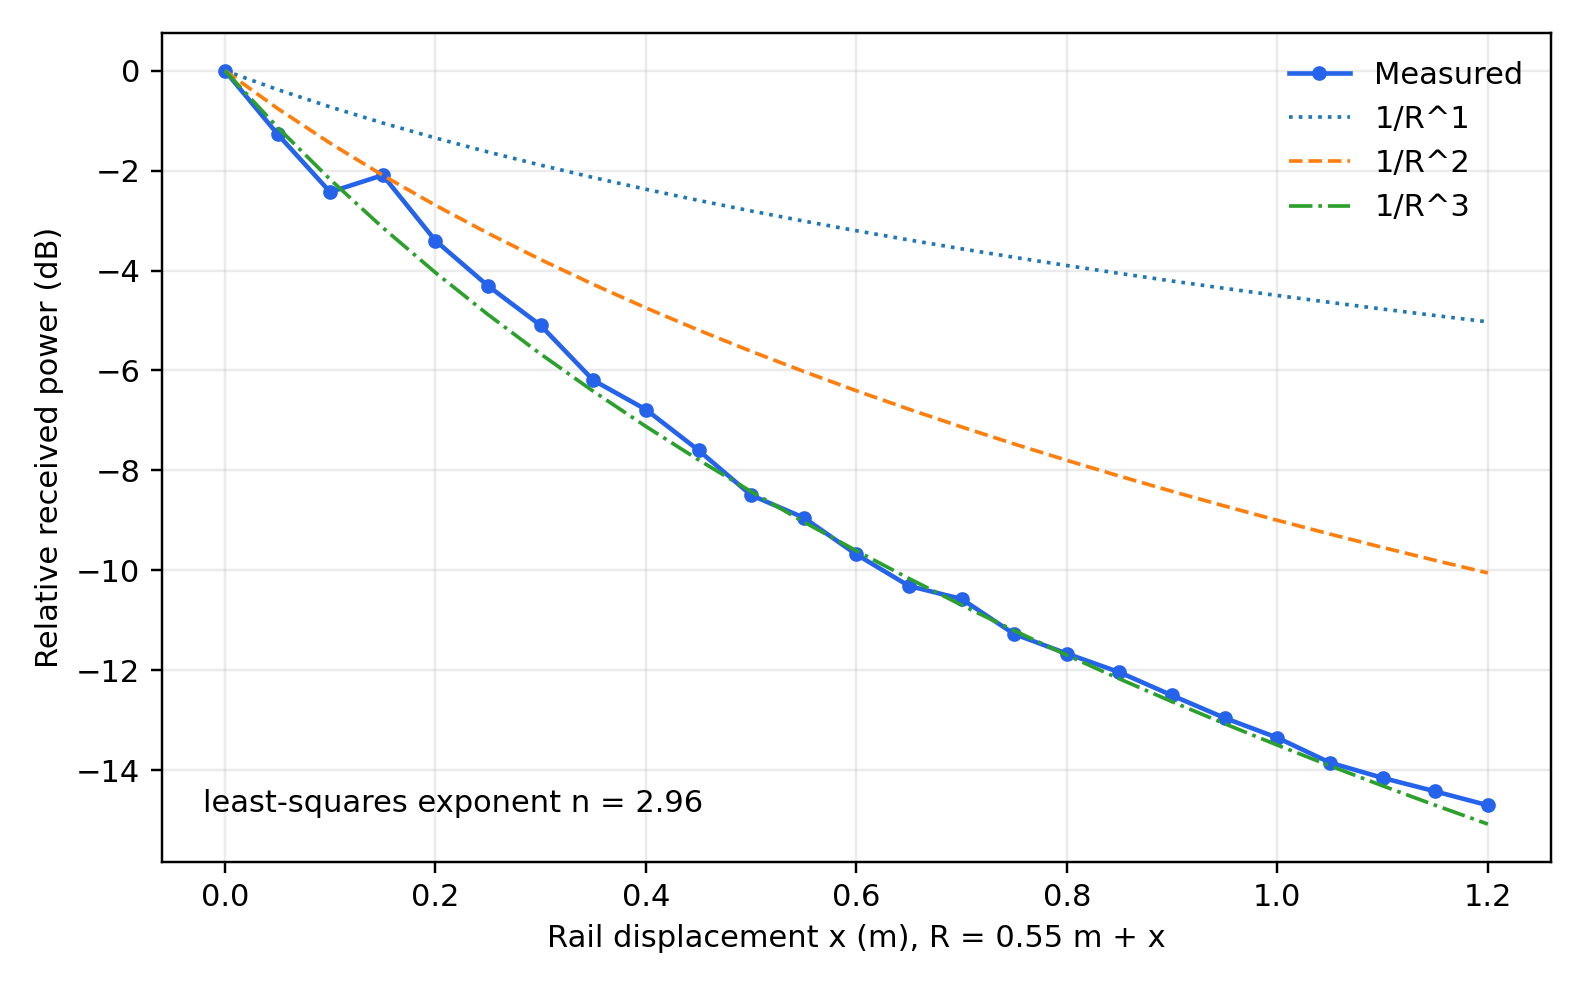
\includegraphics[width=0.74\textwidth]{figures/distance_power_fit.png}
  \caption{8.00 GHz 接收功率随距离变化及幂律拟合}
  \label{fig:distance-fit}
\end{figure}

造成指数偏大的主要原因包括：实验距离只略大于接收喇叭天线的远场判据，场分布仍可能包含近场到远场过渡成分；暗室和周围支架虽有吸波措施，但仍可能产生残余反射；距离改变时接收天线相对主瓣截面的采样位置也随之改变，导致测得量不只是纯粹的球面扩散损耗。

\subsection{远场距离、理论增益与理论波束宽度}

在 8.00 GHz 下，波长
\[
  \lambda=\frac{3.0\times10^8}{8.0\times10^9}=0.0375\,\mathrm{m}.
\]
按指导书的矩形口径判据式 \eqref{eq:far-field-horn} 计算，发射喇叭天线远场距离为
\[
  R_{\mathrm{ff,t,horn}}\approx \frac{2\times0.082\times0.037}{0.0375}=0.162\,\mathrm{m},
\]
接收喇叭天线远场距离为
\[
  R_{\mathrm{ff,r,horn}}\approx \frac{2\times0.141\times0.105}{0.0375}=0.790\,\mathrm{m}.
\]
若进一步按最大线度判据式 \eqref{eq:far-field} 作保守估计，发射天线最大口径取 $D=0.082\,\mathrm{m}$，有
\[
  R_{\mathrm{ff,t}}\approx \frac{2(0.082)^2}{0.0375}=0.359\,\mathrm{m}.
\]
接收天线最大口径取 $D=0.141\,\mathrm{m}$，有
\[
  R_{\mathrm{ff,r}}\approx \frac{2(0.141)^2}{0.0375}=1.060\,\mathrm{m}.
\]
方向图测量中收发天线距离设为约 $1.2\,\mathrm{m}$，大于指导书判据和保守判据下的远场距离，因此可认为满足远场测量条件；但相对接收天线的保守远场距离仅有约 13\% 的余量，实际结果仍可能受过渡区影响。

\begin{table}[H]
  \centering
  \caption{8.00 GHz 下收、发喇叭天线理论参数（取 $k\approx1$）}
  \label{tab:theory-gain}
  \small
  \begin{tabular}{ccccc}
    \toprule
    天线 & $D_E$/cm & $D_H$/cm & 理论增益/dBi & 理论 HPBW：H/E 面 \\
    \midrule
    发射喇叭 & 3.7 & 8.2 & 14.33 & $30.92^\circ/51.68^\circ$ \\
    接收喇叭 & 10.5 & 14.1 & 21.22 & $17.98^\circ/18.21^\circ$ \\
    \bottomrule
  \end{tabular}
\end{table}

发射天线在 $k\approx1$ 理想口径基准下的理论增益为 14.33 dBi，而方向图波束宽度法在 8.5 GHz 给出的实测估计为 13.75 dBi，二者相差约 0.58 dB。若采用指导书中 $k=0.51$ 的保守工程估计，则发射天线和接收天线的增益会分别降低约 2.92 dB，约为 11.41 dBi 和 18.30 dBi。由于波束宽度法本身由实测主瓣宽度反推方向性，后续比较主要采用 $k\approx1$ 的口径基准来观察趋势；实际增益仍会受到口径效率、边缘绕射和装置误差影响。

\subsection{与 CST 仿真结果的对比}

CST 仿真实验采用 CST Studio Suite 2018 建立矩形波导馈电角锥喇叭模型，主要尺寸为 $D_H=80\,\mathrm{mm}$、$D_E=38\,\mathrm{mm}$、$L=80\,\mathrm{mm}$，馈电矩形波导内尺寸为 $a=22.86\,\mathrm{mm}$、$b=10.16\,\mathrm{mm}$，与本实验发射喇叭天线尺寸接近。仿真频段设为 8.2--12.4 GHz，边界采用 open(add space)，端口采用矩形波导端口并以 $\mathrm{TE}_{10}$ 主模激励；远场、场分布和表面电流监视器频率设为 10.3 GHz。由于实测扫频最高到 8.5 GHz，而 CST 远场结果取 10.3 GHz，两者不作逐点数值等同，主要用于趋势和物理机制对照。

\begin{figure}[H]
  \centering
  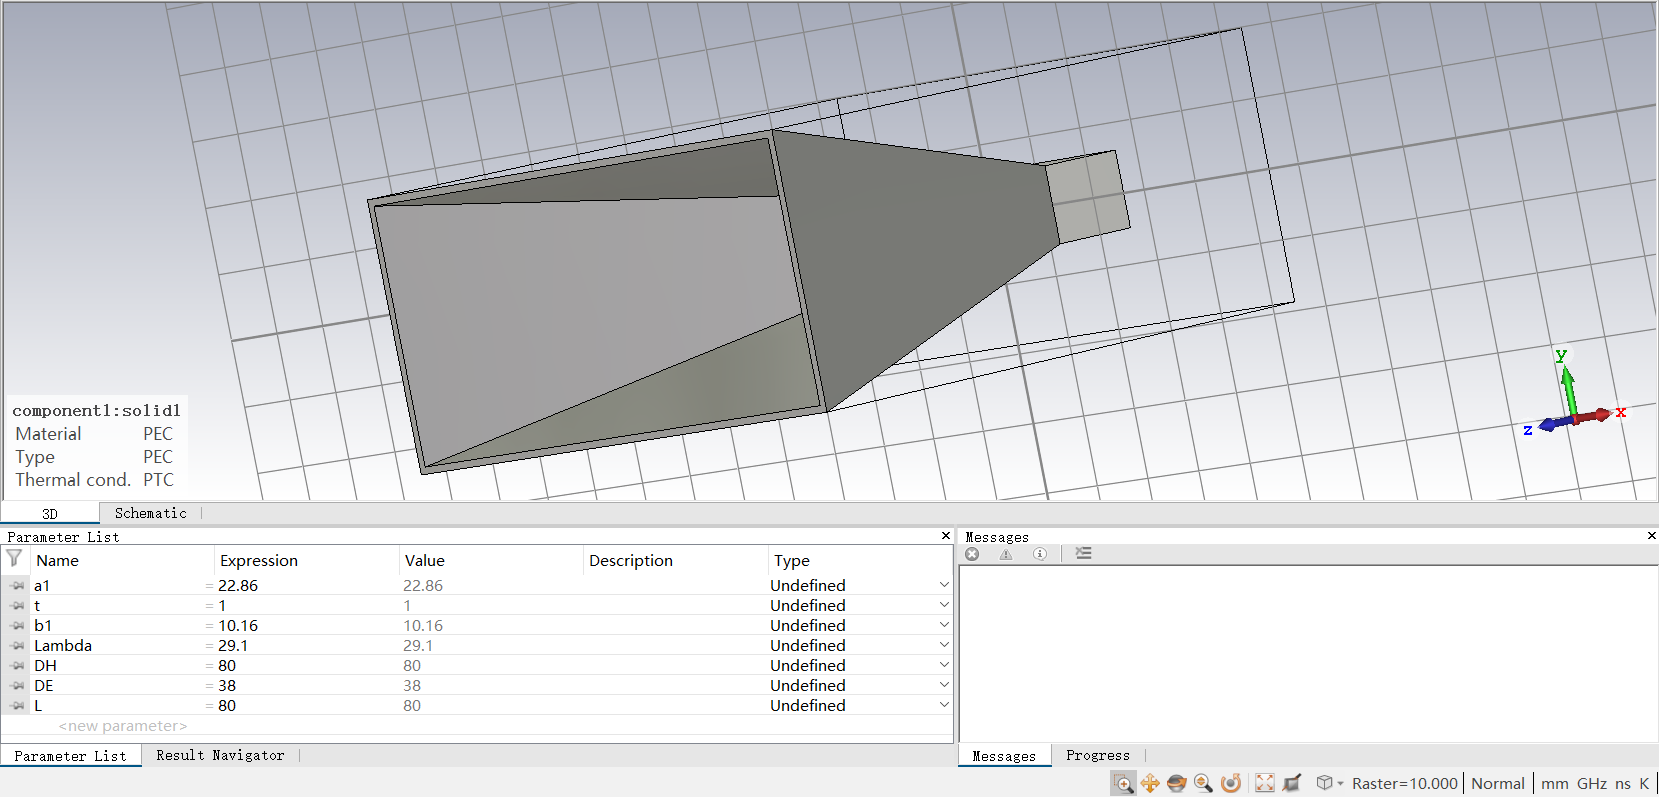
\includegraphics[width=0.82\textwidth]{../../CST仿真/报告源码/figures/矩形波导馈电的角锥喇叭天线 CST 模型.png}
  \caption{矩形波导馈电角锥喇叭天线 CST 参数化模型}
  \label{fig:cst-model}
\end{figure}

图 \ref{fig:cst-model} 中可见，模型由矩形波导、渐变角锥段和开口口径面构成，参数列表中保留了 $a$、$b$、$D_H$、$D_E$、$L$ 和壁厚 $t$，便于后续修改结构尺寸。端口场分布如图 \ref{fig:cst-port-fields} 所示，电场主要沿波导窄边方向分布，宽边中心较强、边缘较弱，符合矩形波导 $\mathrm{TE}_{10}$ 主模特征；图中主模截止频率约为 6.85 GHz，低于 8.2--12.4 GHz 仿真频段。

\begin{figure}[H]
  \centering
  \begin{subfigure}[b]{0.48\textwidth}
    \centering
    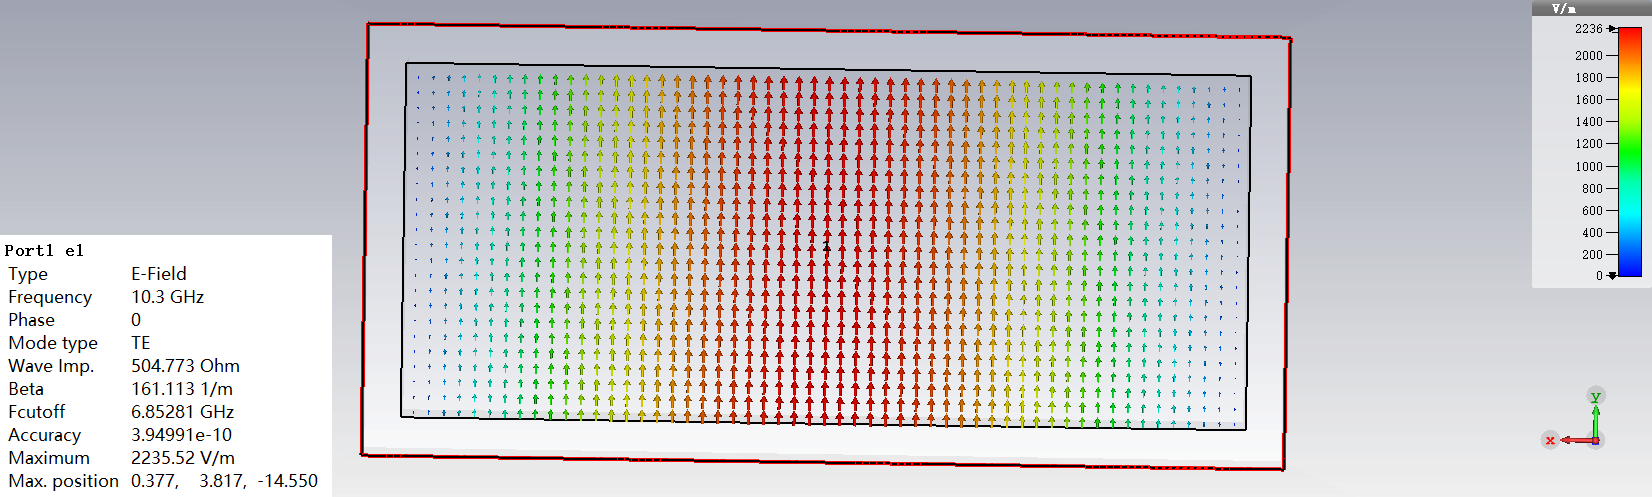
\includegraphics[width=\textwidth]{../../CST仿真/报告源码/figures/e1.png}
    \caption{端口电场分布}
  \end{subfigure}
  \hfill
  \begin{subfigure}[b]{0.48\textwidth}
    \centering
    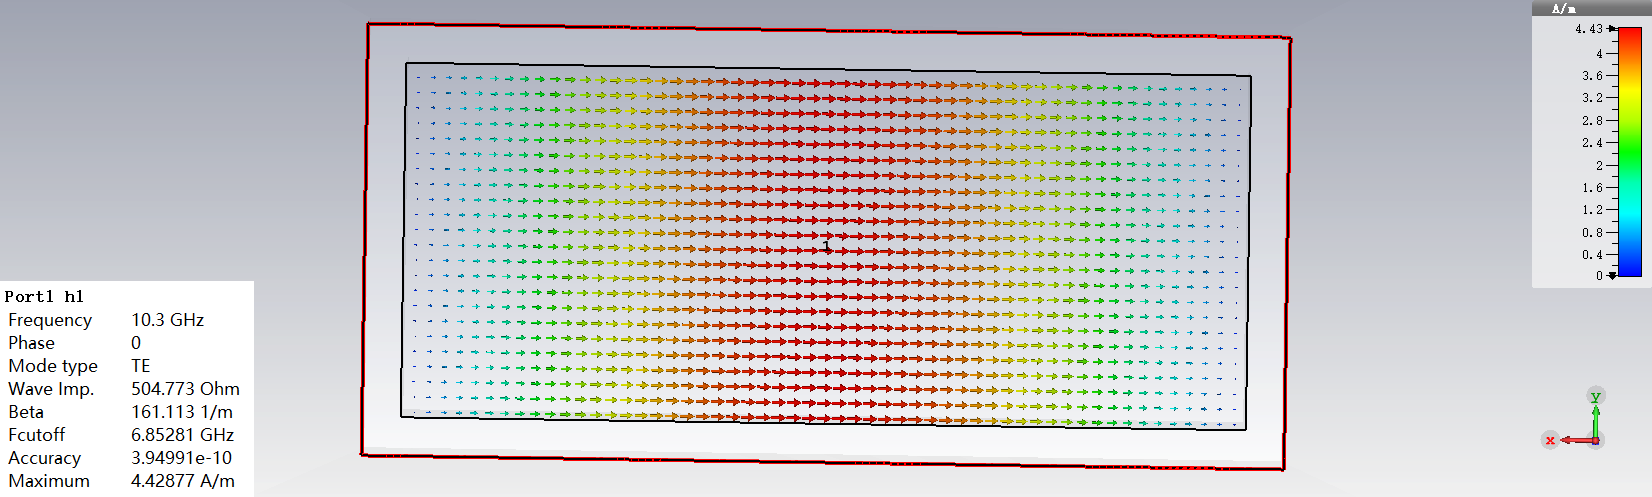
\includegraphics[width=\textwidth]{../../CST仿真/报告源码/figures/h1.png}
    \caption{端口磁场分布}
  \end{subfigure}
  \caption{CST 波导端口 $\mathrm{TE}_{10}$ 模式场分布}
  \label{fig:cst-port-fields}
\end{figure}

仿真的端口匹配结果如图 \ref{fig:cst-sparam} 所示。8.2--12.4 GHz 内 $S_{11}$ 整体约低于 $-20\,\mathrm{dB}$，12.4 GHz 附近下探到约 $-50\,\mathrm{dB}$；VSWR 大部分频点在 1.1 左右，最高约 1.23。这说明该角锥喇叭的渐变结构在 X 波段内具有较好的宽带阻抗变换作用。与实测相比，8.5 GHz 附近实测 VSWR 为 1.099，二者都指向“高频端匹配较好”的结论。

\begin{figure}[H]
  \centering
  \begin{subfigure}[b]{0.48\textwidth}
    \centering
    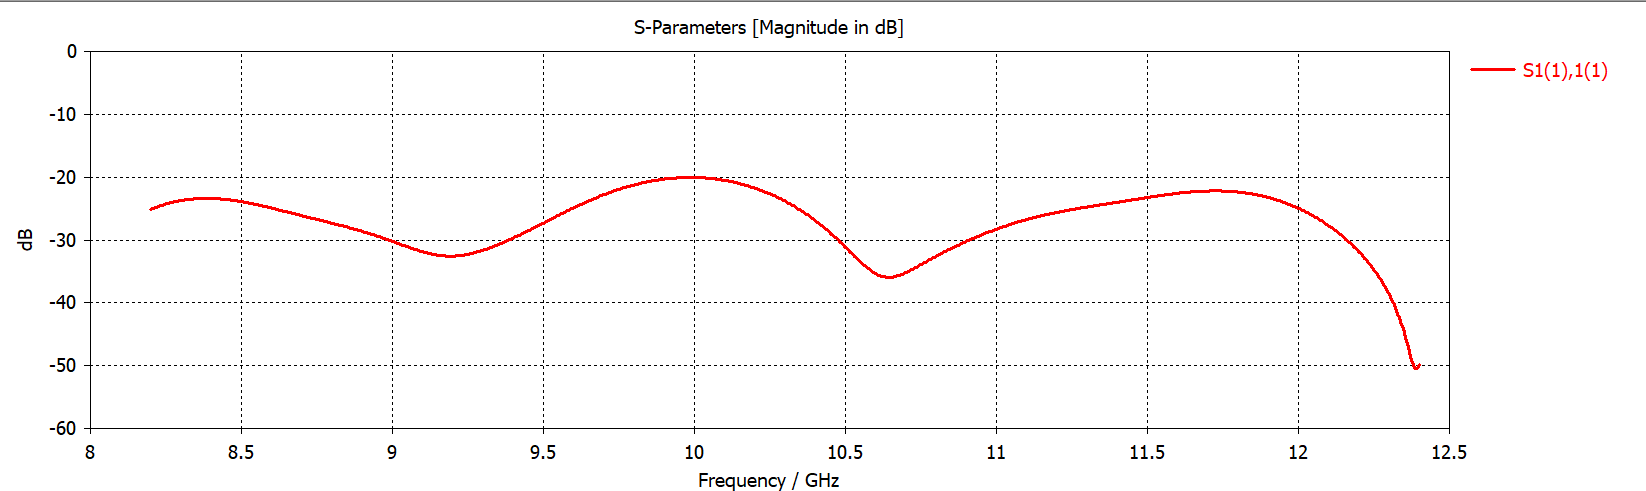
\includegraphics[width=\textwidth]{../../CST仿真/报告源码/figures/S11.png}
    \caption{$S_{11}$ 对数幅度}
  \end{subfigure}
  \hfill
  \begin{subfigure}[b]{0.48\textwidth}
    \centering
    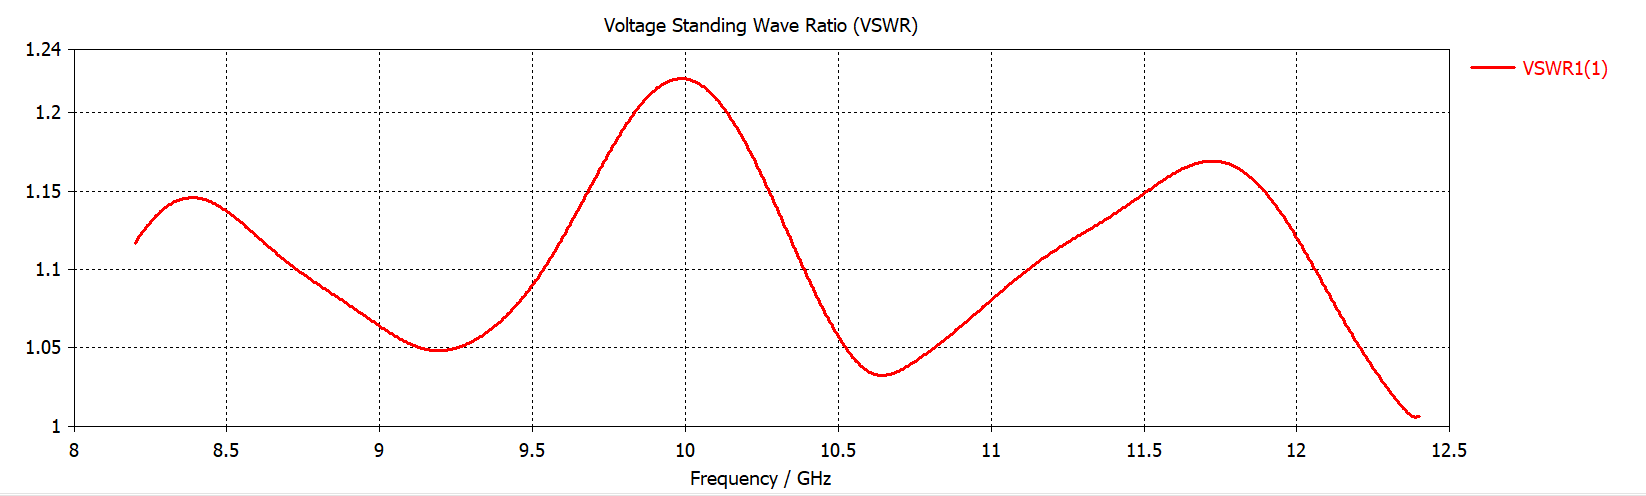
\includegraphics[width=\textwidth]{../../CST仿真/报告源码/figures/VSWR.png}
    \caption{VSWR}
  \end{subfigure}
  \caption{CST 端口匹配仿真结果}
  \label{fig:cst-sparam}
\end{figure}

远场结果如图 \ref{fig:cst-gain} 和图 \ref{fig:cst-pattern-cuts} 所示。10.3 GHz 时最大增益约为 15.04 dB，主瓣沿模型轴向辐射，H 面（$\Phi=0^\circ$）半功率波束宽度约 $26.3^\circ$，E 面（$\Phi=90^\circ$）半功率波束宽度约 $37.3^\circ$。H 面口径尺寸较大，因此 H 面波束更窄；这与实测方向图中 H 面波束小于 E 面波束的趋势一致。

\begin{figure}[H]
  \centering
  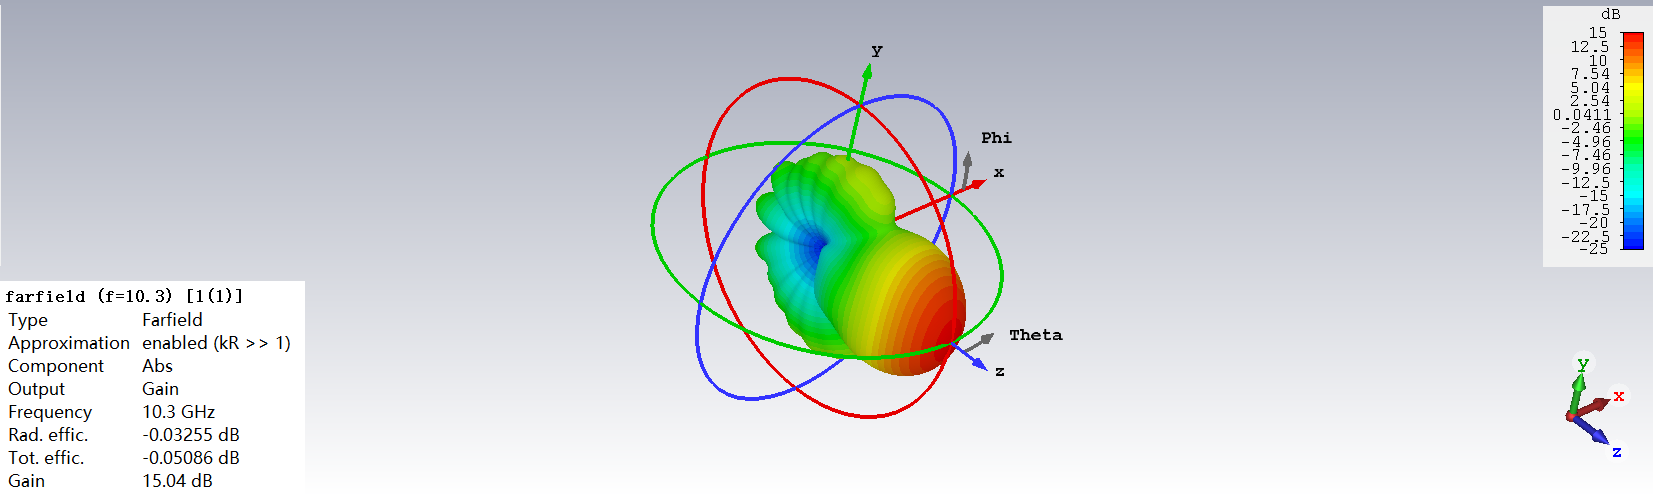
\includegraphics[width=0.78\textwidth]{../../CST仿真/报告源码/figures/增益.png}
  \caption{10.3 GHz CST 三维远场增益分布}
  \label{fig:cst-gain}
\end{figure}

\begin{figure}[H]
  \centering
  \begin{subfigure}[b]{0.48\textwidth}
    \centering
    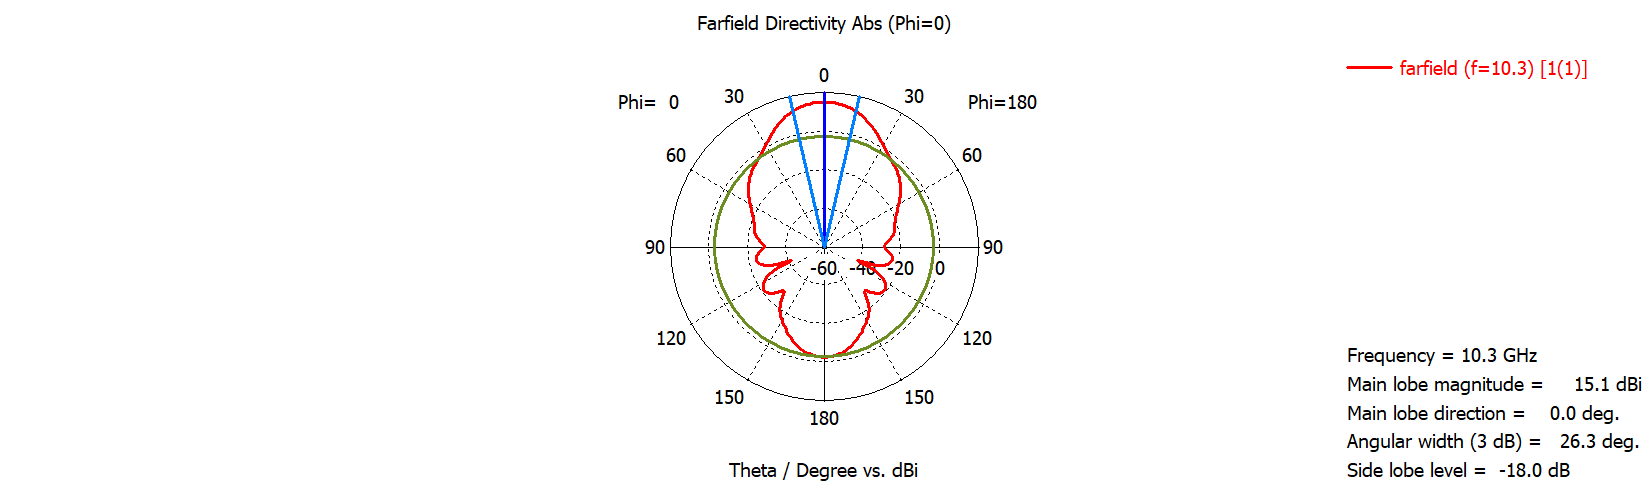
\includegraphics[width=\textwidth]{../../CST仿真/报告源码/figures/0方向图.png}
    \caption{H 面方向图，$\Phi=0^\circ$}
  \end{subfigure}
  \hfill
  \begin{subfigure}[b]{0.48\textwidth}
    \centering
    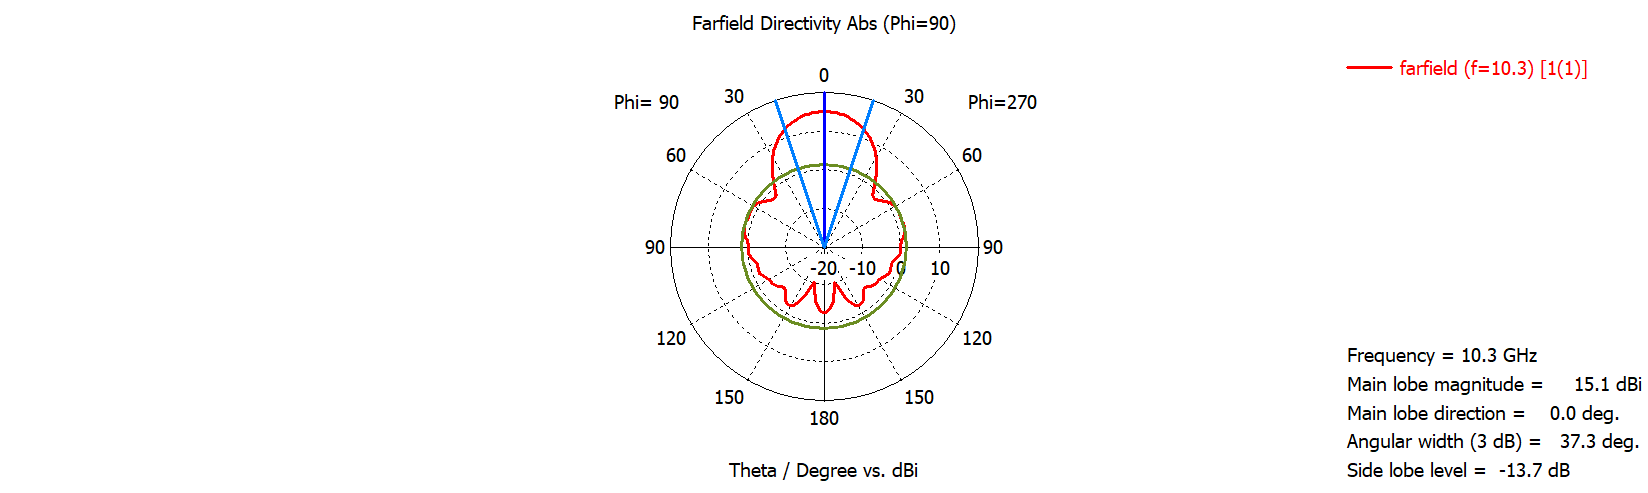
\includegraphics[width=\textwidth]{../../CST仿真/报告源码/figures/90方向图.png}
    \caption{E 面方向图，$\Phi=90^\circ$}
  \end{subfigure}
  \caption{10.3 GHz CST 远场方向图切面}
  \label{fig:cst-pattern-cuts}
\end{figure}

场分布和表面电流结果可进一步解释仿真趋势，如图 \ref{fig:cst-field-current} 所示。波导中的主模进入角锥渐变段后，场分布随横截面扩大而逐渐向口径面展开；表面电流主要集中在波导内壁和喇叭喉部附近，向口径方向逐渐减弱。这与喇叭天线作为阻抗渐变过渡结构的物理图像一致。

\begin{figure}[H]
  \centering
  \begin{subfigure}[b]{0.48\textwidth}
    \centering
    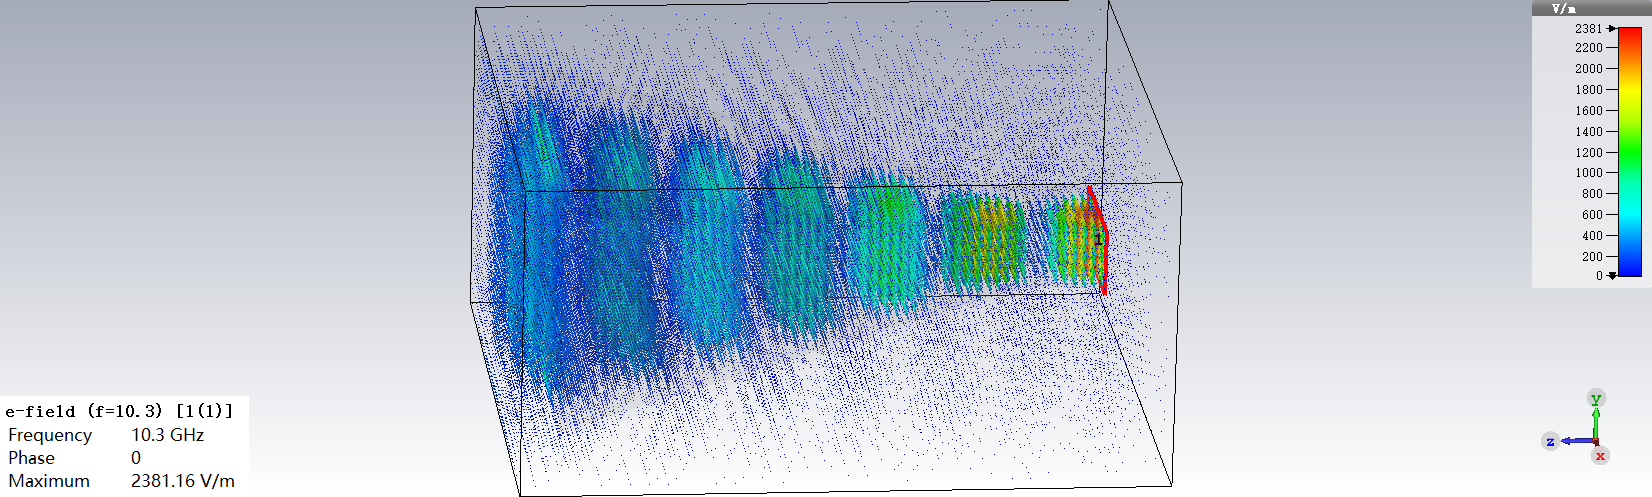
\includegraphics[width=\textwidth]{../../CST仿真/报告源码/figures/电场.png}
    \caption{空间电场分布}
  \end{subfigure}
  \hfill
  \begin{subfigure}[b]{0.48\textwidth}
    \centering
    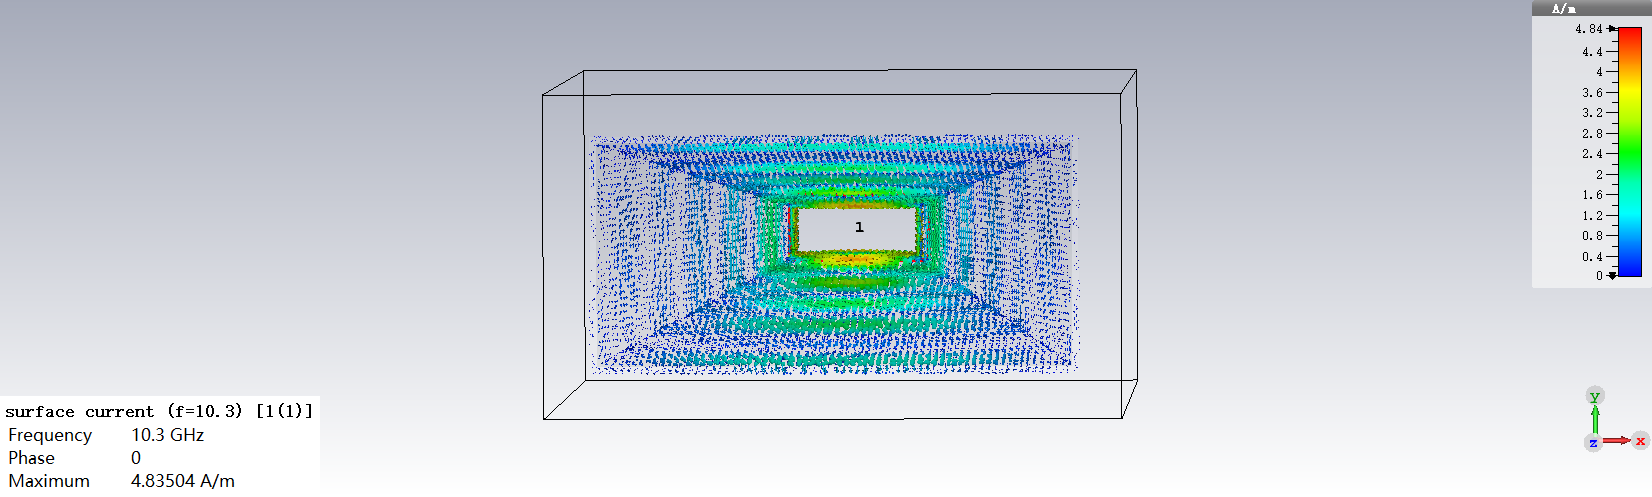
\includegraphics[width=\textwidth]{../../CST仿真/报告源码/figures/表面电流内部.png}
    \caption{内壁表面电流分布}
  \end{subfigure}
  \caption{CST 场分布与表面电流结果}
  \label{fig:cst-field-current}
\end{figure}

\begin{table}[H]
  \centering
  \caption{实测结果与 CST 仿真结果的趋势对比}
  \label{tab:cst-compare}
  \small
  \begin{tabular}{p{0.28\textwidth}p{0.31\textwidth}p{0.31\textwidth}}
    \toprule
    指标 & 实测结果 & CST 仿真结果 \\
    \midrule
    端口匹配 & 8.5 GHz 处 VSWR 为 1.099，回波损耗 26.53 dB & 8.2--12.4 GHz 内 VSWR 最大约 1.23 \\
    主瓣方向 & 水平、垂直方向图主瓣均在 $0^\circ$ 附近 & 主辐射方向沿模型轴向 \\
    半功率波束宽度 & 8.5 GHz：H 面 $28.45^\circ$，E 面 $47.98^\circ$ & 10.3 GHz：H 面 $26.3^\circ$，E 面 $37.3^\circ$ \\
    增益 & 8.5 GHz 波束宽度法约 13.75 dBi & 10.3 GHz 最大增益约 15.04 dBi \\
    副瓣水平 & 实测曲线受暗室反射和噪声底影响，侧向读数有限 & H 面第一副瓣约 $-18.0\,\mathrm{dB}$，E 面第一副瓣约 $-13.7\,\mathrm{dB}$ \\
    \bottomrule
  \end{tabular}
\end{table}

综合来看，仿真和实测都显示该角锥喇叭在高频端匹配较好、主瓣沿轴向、H 面波束较窄。实测 E 面波束宽于 CST 结果，主要与工作频率较低、测量距离余量有限、支架和屏蔽板残余反射以及实际天线加工/安装误差有关；CST 中采用 PEC、开放边界和理想端口激励，环境更接近理想自由空间，因此方向图底部和副瓣更规整。

\section{误差分析与改进措施}

\subsection{主要误差来源}

\textbf{端口与仪器误差。} 网络分析仪、连接电缆和转接头会带来幅度与相位误差。若校准参考面与实际天线端口不完全一致，$S_{11}$ 和 $S_{21}$ 曲线会包含连接结构的附加反射和损耗。

\textbf{机械对准误差。} 喇叭天线方向性较强，收发天线主轴若存在小角度偏差，会直接改变接收功率和方向图主瓣位置。实验中方向图主瓣约在 $1^\circ$ 至 $3^\circ$，说明对准总体较好，但仍非完全零偏。

\textbf{远场距离余量不足。} 接收喇叭的远场距离约 1.060 m，而测量距离约 1.2 m，仅略高于判据。有限距离会使口径相位和空间衰减不完全符合远场近似。

\textbf{环境反射与噪声。} 虽然暗室和吸波材料可降低反射，但滑轨、支架、人员位置、屏蔽板摆放都会影响边界条件。方向图 $\pm90^\circ$ 附近的读数已经接近背景噪声和旁向残余反射的量级，因此不能按理想方向图零点解释。

\textbf{数据采样误差。} 方向图角度步进为 $2^\circ$，极化步进为 $1^\circ$，距离步进为 0.05 m。有限步进会影响主瓣峰值、3 dB 交点和幂律拟合指数的精度。

\subsection{改进措施}

可从以下方面提高测量准确性：测量前进行完整的端口校准和电缆检查，并在报告中记录校准状态；利用激光或机械标尺辅助收发天线轴向对准；方向图测量时适当增大收发距离，使其明显大于较大口径天线的远场距离；保持人员远离主波束和侧向反射路径，固定吸波棉位置；对方向图主瓣附近采用更小角度步进，以提高半功率点插值精度；距离测量时记录真实口面间距而不仅是滑轨位移，减少 $R_0$ 估计带来的不确定性。

\section{专题讨论}

\subsection{收发天线正交并加入 $45^\circ$ 极化栅网时的影响}

若收、发喇叭天线极化方向相差 $90^\circ$，没有栅网时理想接收功率为零。若在两者之间放置相对于发射天线为 $45^\circ$ 的极化栅网，可把发射电场投影到栅网允许透过的方向，再投影到接收天线方向。两次投影的幅度因子均为 $\cos45^\circ$，因此接收场幅度约为
\[
  E_r\propto \cos45^\circ\cos45^\circ=\frac{1}{2},
\]
功率约为
\[
  P_r\propto \left(\frac{1}{2}\right)^2=\frac{1}{4},
\]
相当于比同极化理想接收低 $6.02\,\mathrm{dB}$。实际测量中还会叠加栅网损耗、反射和交叉极化泄漏，因此读数不会严格等于该值。

\subsection{收发天线相同时的简便增益测量}

当收发天线型号、尺寸和安装状态相同，可令 $G_t=G_r=G$，由式 \eqref{eq:friis} 得
\begin{equation}
  G(\mathrm{dBi})=\frac{1}{2}\left[P_r(\mathrm{dBm})-P_t(\mathrm{dBm})
  +20\log_{10}\left(\frac{4\pi R}{\lambda}\right)\right].
  \label{eq:same-antenna-gain}
\end{equation}
这种方法不需要额外标准增益天线，适合教学实验。为减小系统误差，应保持收发天线严格同轴、同极化，测量前扣除电缆和转接头损耗，保证距离满足远场条件，并通过交换两副天线位置或多距离测量取平均值来削弱单次安装误差。

\subsection{$\pm90^\circ$ 方向图读数的解释}

理想角锥喇叭在主轴侧向方向的辐射应显著低于主瓣，但实验方向图在 $\pm90^\circ$ 附近仍有有限读数。这部分读数并不代表天线在侧向存在强有效辐射，而是由副瓣、交叉极化分量、暗室残余反射、支架散射和接收机噪声底共同决定。当主瓣外信号已经降至几十 dB 以下时，背景噪声和多径分量会抬高曲线底部，使实测方向图难以继续下降到理论零值。

\section{实验报告内容要求完成情况}

根据实验指导书的报告要求，本文各项处理与结论归纳如下。

\begin{enumerate}
  \item \textbf{误差来源与改进措施。} 处理过程见第 5 节。主要误差来自端口校准、机械对准、远场距离余量、环境反射与采样步进；提高精度的关键是完整校准、精确对轴、增大测量距离、固定吸波材料位置并细化主瓣附近采样。
  \item \textbf{距离传播曲线与衰减规律。} 处理过程见第 4.4 节。8.00 GHz 下，接收功率随距离变化的拟合指数约为 $n=2.96$，在本实验平台上更接近 $1/R^3$ 衰减；其偏离理想 $1/R^2$ 的原因主要是有限距离、残余反射和近远场过渡影响。
  \item \textbf{极化曲线及极化规律。} 处理过程见第 4.3 节。常规极化曲线随极化角增大而下降，整体接近 $20\log_{10}|\cos\alpha|$；若从接收功率角度表述，则近似满足 $\cos^2\alpha$ 关系。加入极化栅网后，接收幅度进一步降低，说明栅网引入了额外透射损耗和散射。
  \item \textbf{极化思考题。} 处理过程见第 6.1 节。收发天线正交时理论接收为零；加入相对发射极化方向 $45^\circ$ 的栅网后，两次场投影使接收功率约为同极化理想值的 $1/4$，即低约 $6.02\,\mathrm{dB}$。
  \item \textbf{远区场距离判断。} 处理过程见第 4.5 节。按指导书矩形口径判据，发射和接收喇叭远场距离约为 0.162 m 和 0.790 m；按最大线度保守判据分别约为 0.359 m 和 1.060 m。方向图测量距离约 1.2 m，满足远场条件，但相对接收天线的保守判据余量有限。
  \item \textbf{理论增益与半功率波束宽度。} 处理过程见第 4.5 节。8.00 GHz 下，发射喇叭理想口径基准增益约 14.33 dBi，理论 H/E 面 HPBW 为 $30.92^\circ/51.68^\circ$；接收喇叭对应增益约 21.22 dBi，理论 H/E 面 HPBW 为 $17.98^\circ/18.21^\circ$。
  \item \textbf{方向图绘制与整体性能评价。} 处理过程见第 4.2 节。6.5、7.5、8.5 GHz 三个频点的水平面和垂直面方向图主瓣均在 $0^\circ$ 附近，说明轴向对准较好；频率升高时 H 面波束变窄，方向性增强。
  \item \textbf{理论与实测半功率波束宽度对比。} 处理过程见第 4.2 节。H 面理论值与实测值吻合较好，8.5 GHz 处仅相差约 $0.65^\circ$；E 面整体也符合口径越小波束越宽的规律，局部偏差与角度步进、反射和对准误差有关。
  \item \textbf{收发天线相同时的简便增益测量。} 处理过程见第 6.2 节。由弗里斯公式可在 $G_t=G_r$ 时反推出单副天线增益；减小系统误差需扣除链路损耗、保证同轴同极化、满足远场条件，并通过交换天线位置或多距离平均削弱安装误差。
  \item \textbf{$\pm90^\circ$ 方向图读数解释。} 处理过程见第 6.3 节。侧向读数主要由副瓣、交叉极化、暗室残余反射、支架散射和噪声底共同决定，不能按理想零辐射直接解释。
  \item \textbf{实测与 CST 仿真对比。} 处理过程见第 4.6 节。实测与仿真均显示高频端匹配较好、主瓣沿轴向、H 面波束较窄；由于实测最高频点为 8.5 GHz，而 CST 远场监视器为 10.3 GHz，数值比较以趋势为主。
  \item \textbf{实验收获与流程改进。} 综合第 4 节至第 6 节可知，端口匹配、口径尺寸、极化方向和测量距离共同决定空间链路测量结果。后续实验应重点记录真实口面间距、校准状态和屏蔽板位置，以便进一步减小系统误差。
\end{enumerate}

\section{实验结论与体会}

本次实验完成了波导角锥喇叭天线的 $S$ 参数、方向图、极化和距离传播特性测量。$S_{11}$ 结果表明，发射喇叭在 7.5 GHz 以上匹配明显改善，最低 VSWR 为 1.069；$S_{21}$ 在 7.0 GHz 以后进入较稳定传输区，说明该频段内收发链路更适合后续辐射特性测量。方向图测量表明，主瓣位于轴向附近，8.5 GHz 处 H 面和 E 面半功率波束宽度分别为 $28.45^\circ$ 和 $47.98^\circ$，H 面波束较窄，符合 H 面口径较大的结构特征；波束宽度法估计增益为 13.75 dBi，与理论口径估算处于同一量级。极化测量验证了线极化投影规律，接收功率随极化角近似服从 $\cos^2\alpha$；距离测量在本实验平台上更接近 $1/R^3$ 衰减，反映出有限测量距离、环境反射和近远场过渡对理想自由空间模型的影响。

实测结果与 CST 仿真结果在主要趋势上相互印证。CST 模型在 8.2--12.4 GHz 内具有较好的端口匹配，VSWR 最大约 1.23；实测 8.5 GHz 处 VSWR 为 1.099，也表现出良好匹配。CST 在 10.3 GHz 得到的主瓣沿轴向辐射，H 面和 E 面半功率波束宽度约为 $26.3^\circ$ 和 $37.3^\circ$，最大增益约 15.04 dB；实测 8.5 GHz 下 H 面和 E 面半功率波束宽度为 $28.45^\circ$ 和 $47.98^\circ$，波束宽度法增益约 13.75 dBi。由于两者工作频点、边界条件和环境复杂度不同，数值不宜直接逐项等同，但“高频端匹配较好、主瓣沿轴向、H 面波束较窄、增益约为十几 dBi”的结论是一致的。实测 E 面波束更宽，主要与频率较低、远场距离余量有限、支架和屏蔽板残余反射以及实际安装误差有关。

从课程学习角度看，本实验把电磁场与电磁波理论中的若干概念具体化了。驻波比和回波损耗不再只是传输线公式，而是直接反映端口能量是否有效进入天线；弗里斯公式和远场判据说明了测量距离、口径尺寸和波长之间的关系；方向图和半功率波束宽度体现了口径越大、主瓣越窄的辐射规律；极化实验则把电场矢量投影与接收功率的关系直接呈现在曲线上。结合 CST 中的 $\mathrm{TE}_{10}$ 端口场、远场方向图和表面电流分布，可以更直观地理解波导模式如何经喇叭渐变结构过渡并向自由空间辐射。

通过本次实验，可以看到天线参数并不是孤立读数：端口匹配影响可用频段，口径尺寸决定方向图宽度，极化方向决定接收投影，测量距离和环境又会改变空间链路的实际衰减。后续若继续改进实验，可重点提高远场距离裕量、角度对准精度和环境反射控制，并在数据记录中同步保存校准状态、屏蔽板位置和真实口面间距。这样不仅能减小单次测量误差，也能使实测、理论估算和 CST 仿真之间的比较更加可靠。

\end{document}
